\documentclass[12pt, a4paper]{article}

\usepackage[utf8]{inputenc}
\usepackage[T2A]{fontenc}
\usepackage[russian]{babel}
\usepackage[]{float}

\usepackage[oglav, boldsect, eqwhole, figwhole, %
   remarks, hyperref, hyperprint]{fn2kursstyle}

\frenchspacing
\righthyphenmin=2

%Командна для римских прописных 
\newcommand{\RomanNumeralCaps}[1]
    {\MakeUppercase{\romannumeral #1}}

\title{Решение задач интерполирования}
\group{ФН2-52Б}
\author{A.\,И.~Токарев}
\secauthor{Ю.\,А.~Сафронов}
\supervisor{}
\date{2021}

\def\hmath$#1${\texorpdfstring{{\rmfamily\textit{#1}}}{#1}}

\begin{document}
\maketitle
\tableofcontents 
\newpage

\section{Краткое описание алгоритмов}

\subsection{Равномерная сетка}

Шаг равномерной сетки постоянный и вычисляется по формуле: 

\[
    h = \dfrac{b - a}{n},  
\]

\noindent а сами узлы имеют координаты 

\[
    x_i = a + h \cdot i = a + \dfrac{b - a}{n} \cdot i, \quad i = 0,1,\ldots,n
\]

\subsection{Чебышевская сетка}

Узлы вычисляются, как корни многочлена Чебышева $1-$го рода, то есть точки 

\[
    x_i = \dfrac{a + b}{2} + \dfrac{b - a}{2} \cos \dfrac{(2i + 1) \pi }{2 (n + 1)}, \quad i = 0,1,\ldots,n
\]

\subsection{Задача интерполирования}

Задан отрезок $[a, b]$. Пусть точки $x_0 \ldots x_n$ –- узлы интерполяции, то есть точки, лежащие внутри этого отрезка. А значения $y(x_0) = y_0,\  \ldots \  ,y(x_n) = y_n$ -- значения искомой функции в этих точках. Послодовательность $\{y_i\}_{i=0}^n$ будем называть сеточной функцией. 

Таким образом, задача интреполирования заключается в построении такой функции $ f(x) $, которая будет принимать в узлах те же значения, что и $ y_i $. Геометрически это можно интерпретировать, как построение кривой, проходящей через систему точек $ (x_i, y_i) $

\subsection{Многочлен Лагранжа}

Многочлен $n$-степени вида
\[
    L_n(x) = \displaystyle \sum_{k = 0}^{n} \alpha_kx_k,  
\]

\noindent называют { \bf интерполяционным многочленом }, если 
\[
    L_n(x_i) = y_i   
\]

\pagebreak
{ \bf Интерполяционный многочлен Лагранжа }:

\[
    L_n(x) = \displaystyle \sum_{k = 0}^{n} c_k(x)y_k, \quad i = 0,1,\ldots,n
\]

В соответствии с определением интерполяционного полинома получаем:
\[
    \displaystyle \sum_{k = 0}^{n} c_k(x_i)y_k = y_i, \quad c_k(x_i) =  
    \begin{cases}
        0 & i \neq k \\
        1 & i = k
    \end{cases}, \quad i = 0,1,\ldots,n
\]

\subsection{Кубический сплайн}

Кубическим сплайном для функции $y(x)$ называют функцию $S(x)$, удовлетворяющую следующим условиям:

\begin{enumerate}
    \item на каждом отрезке $ [x_{i - 1}, x_{i}] $ функция $S(x)$ –- многочлен третьей степени;
    \item функция $S(x)$, ее первая и вторая производные непрерывны на отрезке $[x_0, x_n]$;
    \item значения функции $S(x)$ и исходной функции $y(x)$ совпадают в узлах интерполяции.
\end{enumerate}

На каждом из отрезков $ [x_{i - 1}, x_{i}] $ функция $S(x) = s_i$ ищется следующим образом 
\[
    s_i = a_i + b_i(x - x_i) + c_i(x - x_i)^2 + d_i(x - x_i)^3 = a_i + b_i h_i + c_i h_i^2 + d_i h_i^3, 
\]

\noindent где $a_i, b_i, c_i, d_i $ -- коэффициенты, подлежазие определению.
\[
    \begin{split}
        & a_i = y_{i - 1}\\
        & a_i + b_i h_i + c_i h_i^2 + d_i h_i^3 = y_i
    \end{split}
\]

Из условия непрерывности первой и второй производной получаем
\[
    \begin{split}
        S^'(x_i - 0) & = S^'(x_i + 0)  \\
        S^{''}(x_i - 0) & = S^{''}(x_i + 0), \quad i = 1, 2, \ldots, n - 1,
    \end{split} 
\]

\noindent тогда 
\[
    \begin{split}
        b_i + 2 c_i h_i + 3 d_i h_i^2 & = b_{i + 1} \\
        2 c_i + 6 d_i h_i & = 2 c_{i + 1}
    \end{split} 
\]

\pagebreak

Положим $ S^{''}(x_0) = S^{''}(x_n) = 0 $, тогда
\[
    \begin{split}
        &2 c_1 = 0 \\ 
        &2 c_n + 6 d_n h_n = 2 c_{n + 1} = 0
    \end{split}   
\]

Введением вспомогательного параметра $ g_i = \dfrac{y_i - y_{i-1}}{h_i} $ получаем систему
\[
  \begin{cases}
    c_1 = 0 \\
    h_{i - 1} c_{i - 1} + 2 (h_{i - 1} + h_i) c_i + h_i c{i + 1} = 3(g_i - g{i - 1}) \\
    c_{n + 1} = 0,
  \end{cases}  
\]

\noindent которая является трехдиагональной и обладает диагональным преобладанием, поэтому для нахождения коэффициентов можно использовать метод прогонки.

Остальные коэффициенты находим по формулам
\[
    \begin{split}
        b_i &= g_i  - \dfrac{(c_{i + 1} + 2 c_i) h_i}{3} \\ 
        d_i &= \dfrac{c_{i + 1} - c_i}{3 h_i}, \quad i = 1, 2, \ldots, n
    \end{split} 
\]


\section{Исходные данные}

\newpage

\section{Результаты расчетов}

\subsection{Первый пункт}

% Равномерная сетка
\begin{figure}[h]
    \center{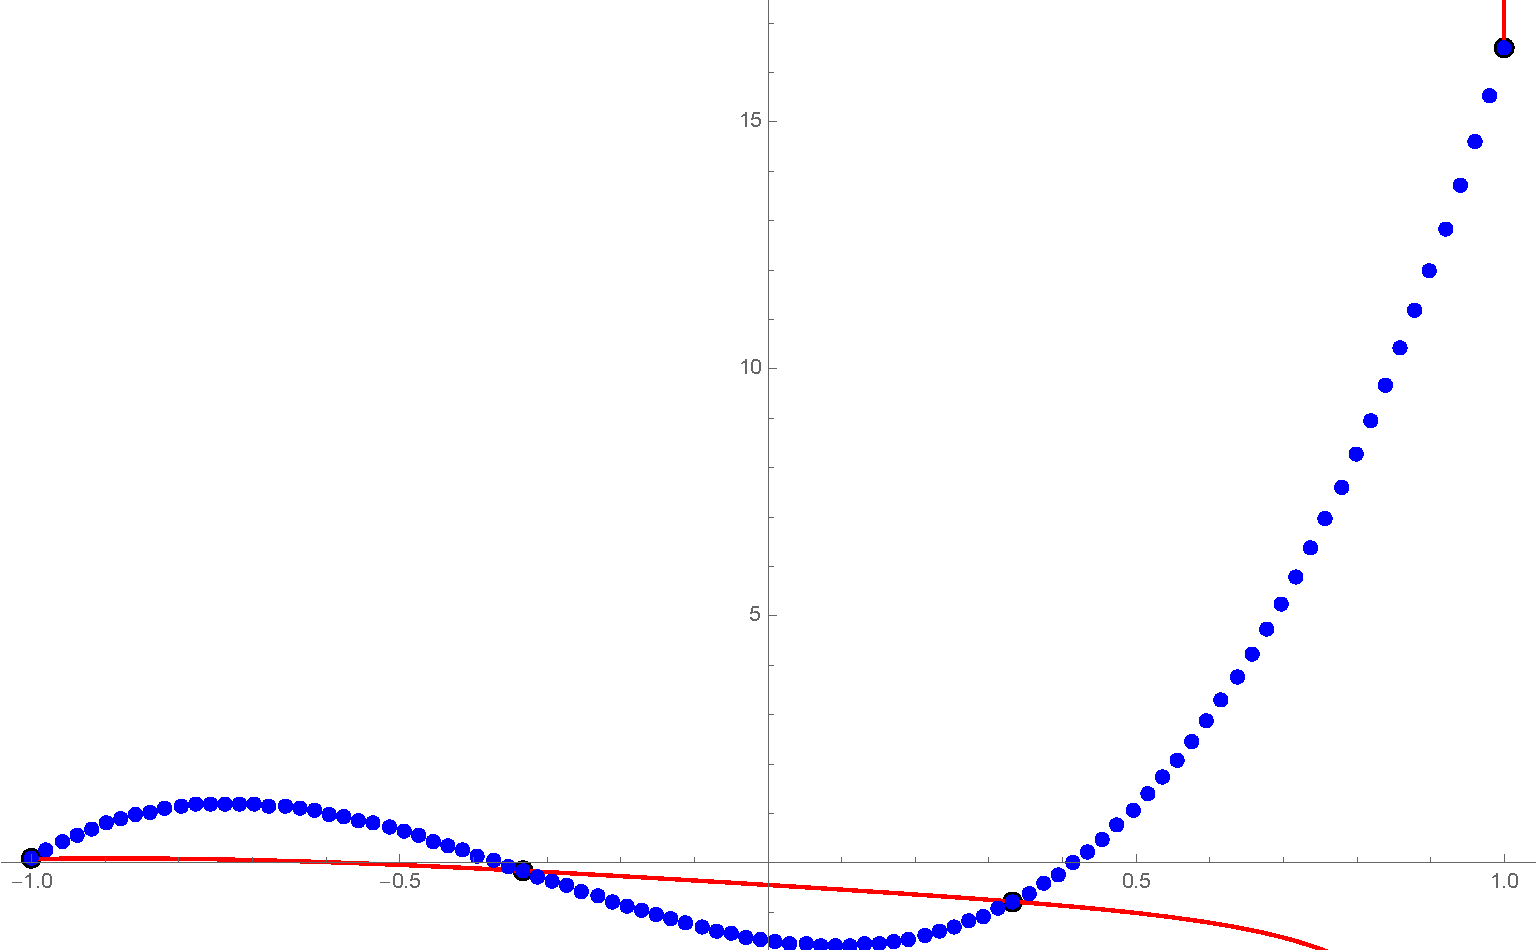
\includegraphics[width=0.8\linewidth]{pic/1/n_4_U.pdf}}
    \caption{Равномерная сетка, $n = 2$, $ \| f(x) - L_n(x)  \|_C = 68.31 $.}
\end{figure}

\begin{figure}[h]
    \center{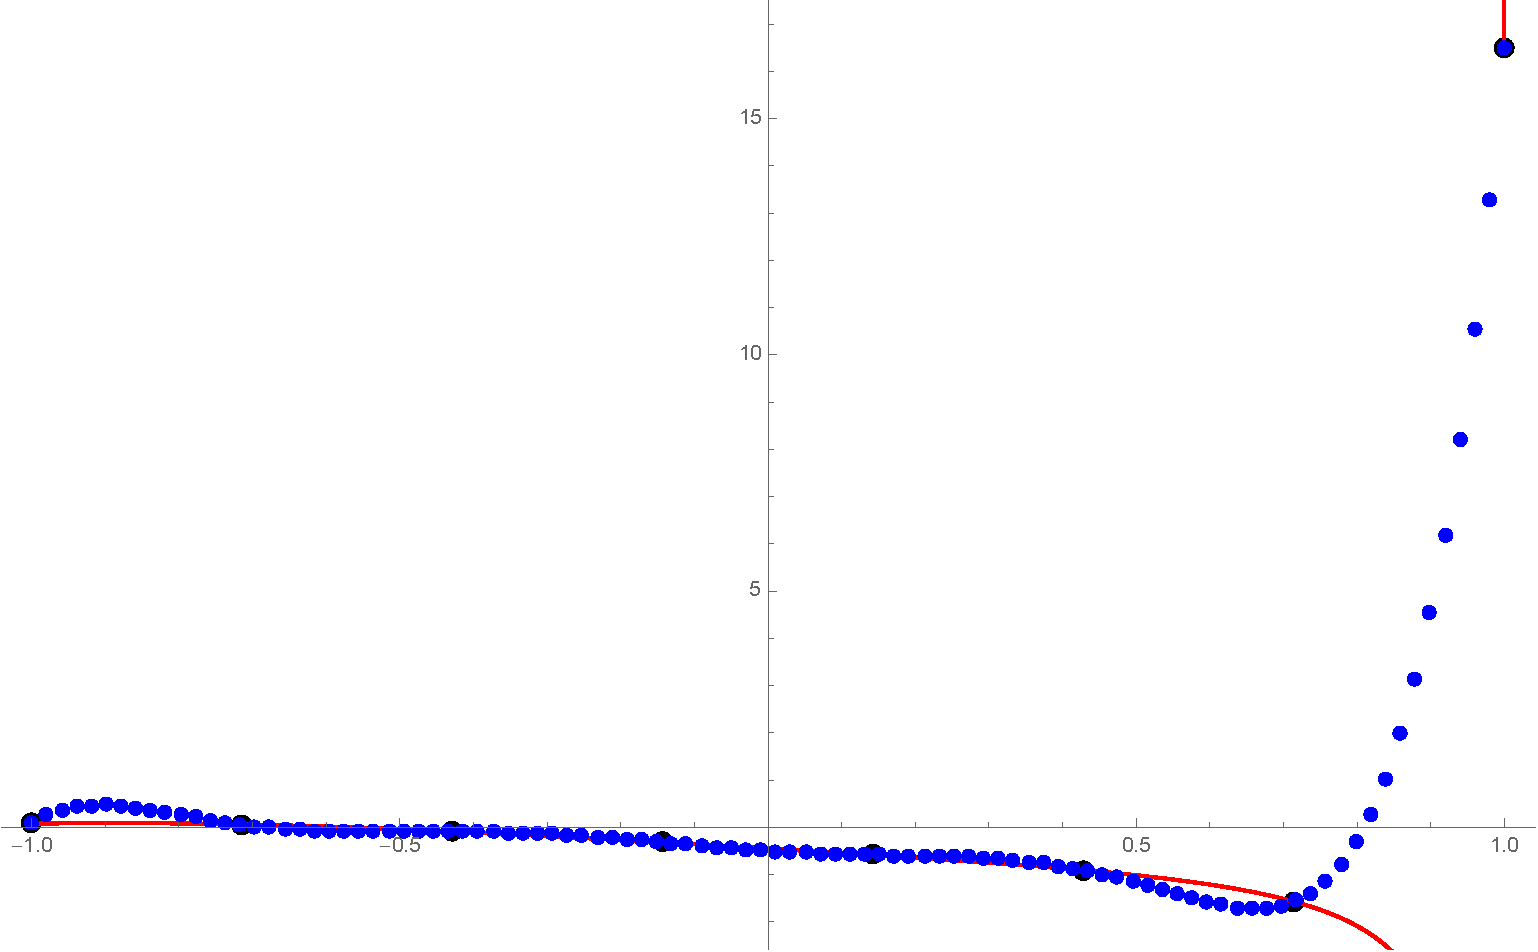
\includegraphics[width=0.8\linewidth]{pic/1/n_8_U.pdf}}
    \caption{Равномерная сетка, $n = 8$, $ \| f(x) - L_n(x)  \|_C = 64.25 $.}
\end{figure}

\pagebreak


\begin{figure}[h]
    \center{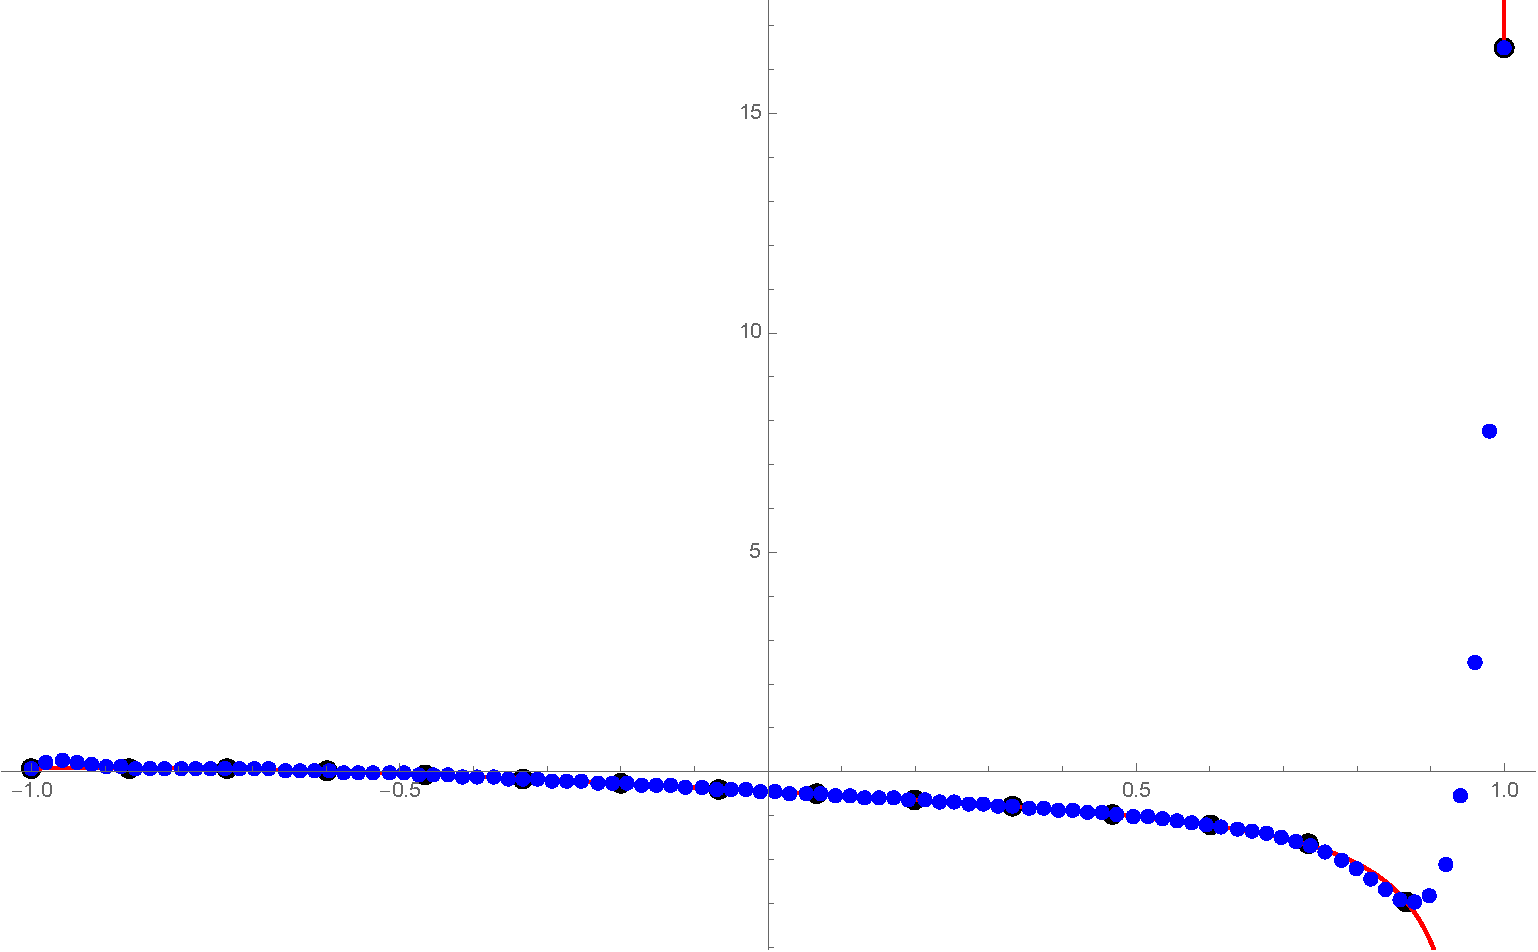
\includegraphics[width=0.8\linewidth]{pic/1/n_16_U.pdf}}
    \caption{Равномерная сетка, $n = 16$, $ \| f(x) - L_n(x)  \|_C = 56.1911 $.}
\end{figure}

\begin{figure}[h]
    \center{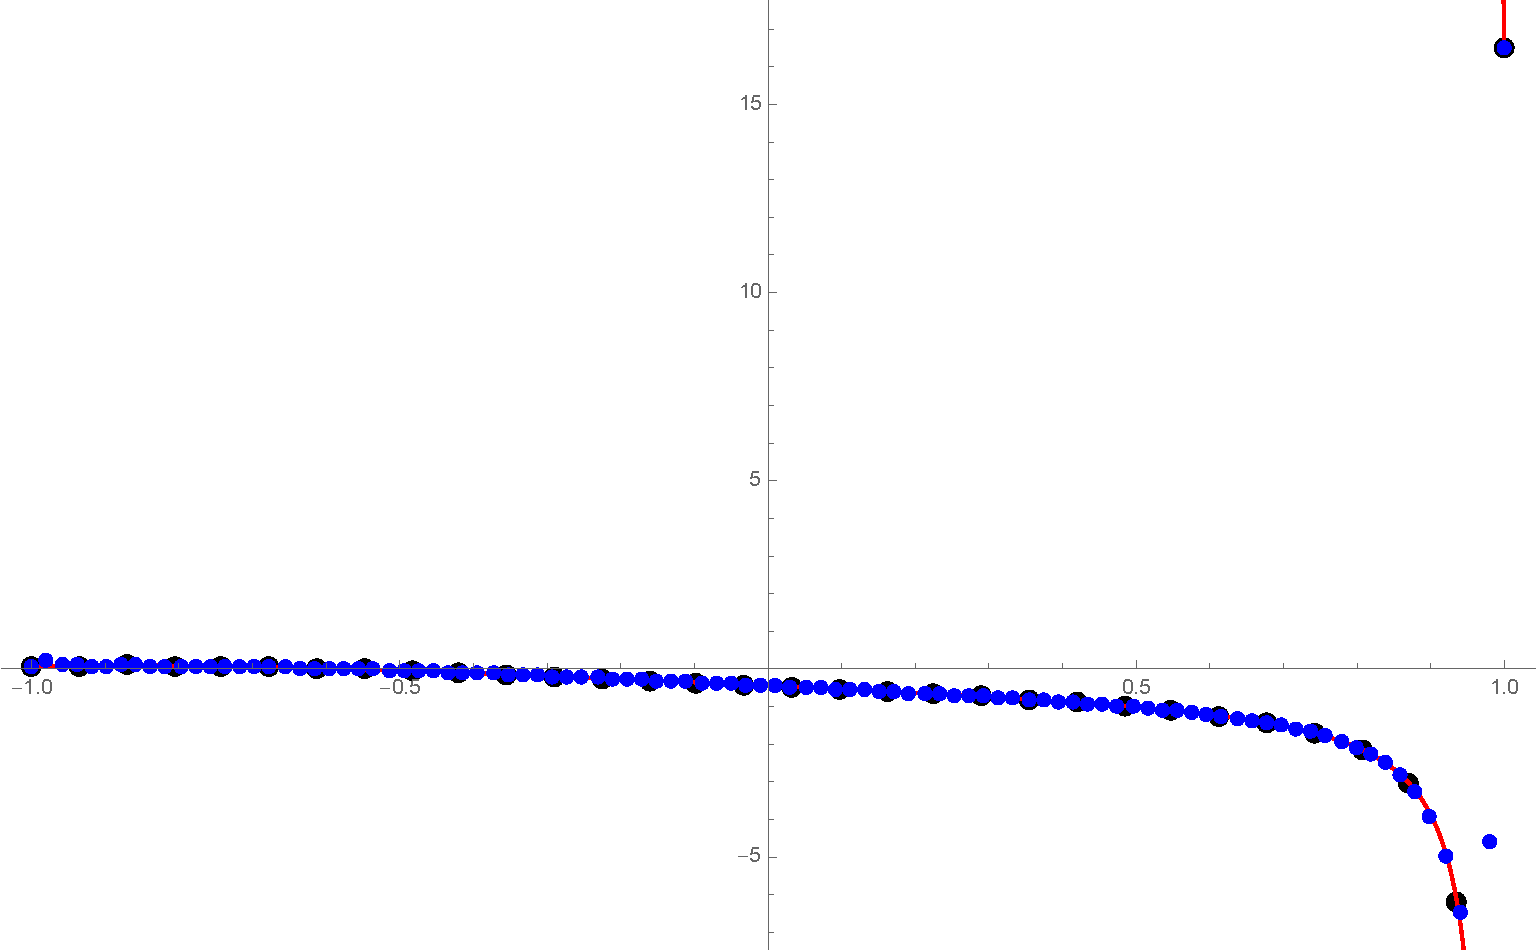
\includegraphics[width=0.8\linewidth]{pic/1/n_32_U.pdf}}
    \caption{Равномерная сетка, $n = 32$, $ \| f(x) - L_n(x)  \|_C = 46.0322 $.}
\end{figure}

\pagebreak


\begin{figure}[h]
    \center{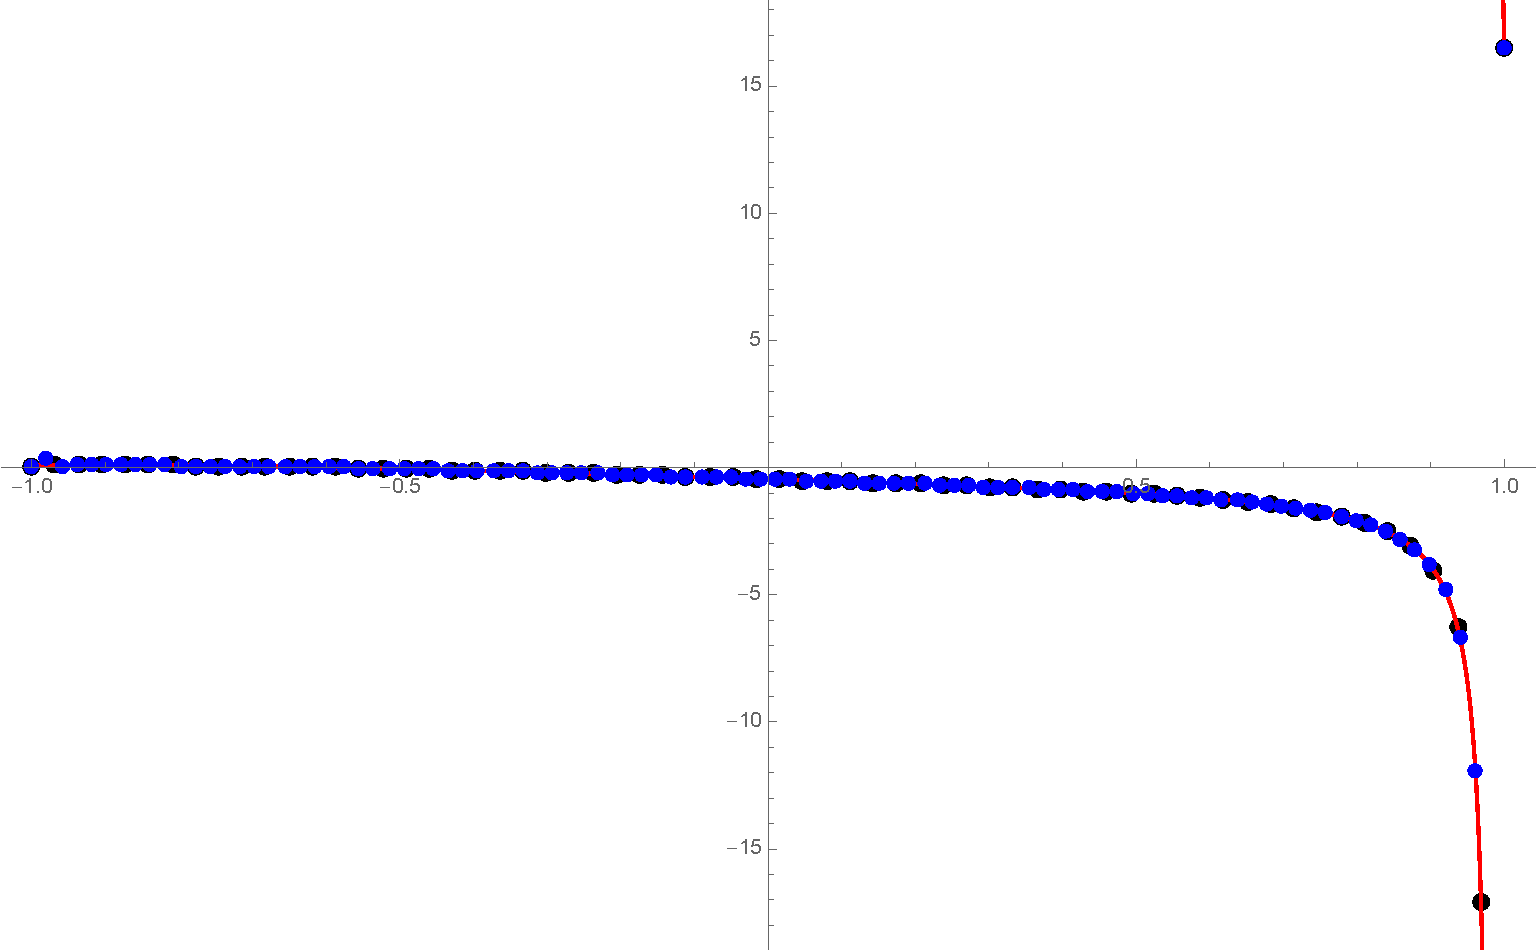
\includegraphics[width=0.8\linewidth]{pic/1/n_64_U.pdf}}
    \caption{Равномерная сетка, $n = 64$, $ \| f(x) - L_n(x)  \|_C = 44.5913 $.}
\end{figure}

\begin{figure}[h]
    \center{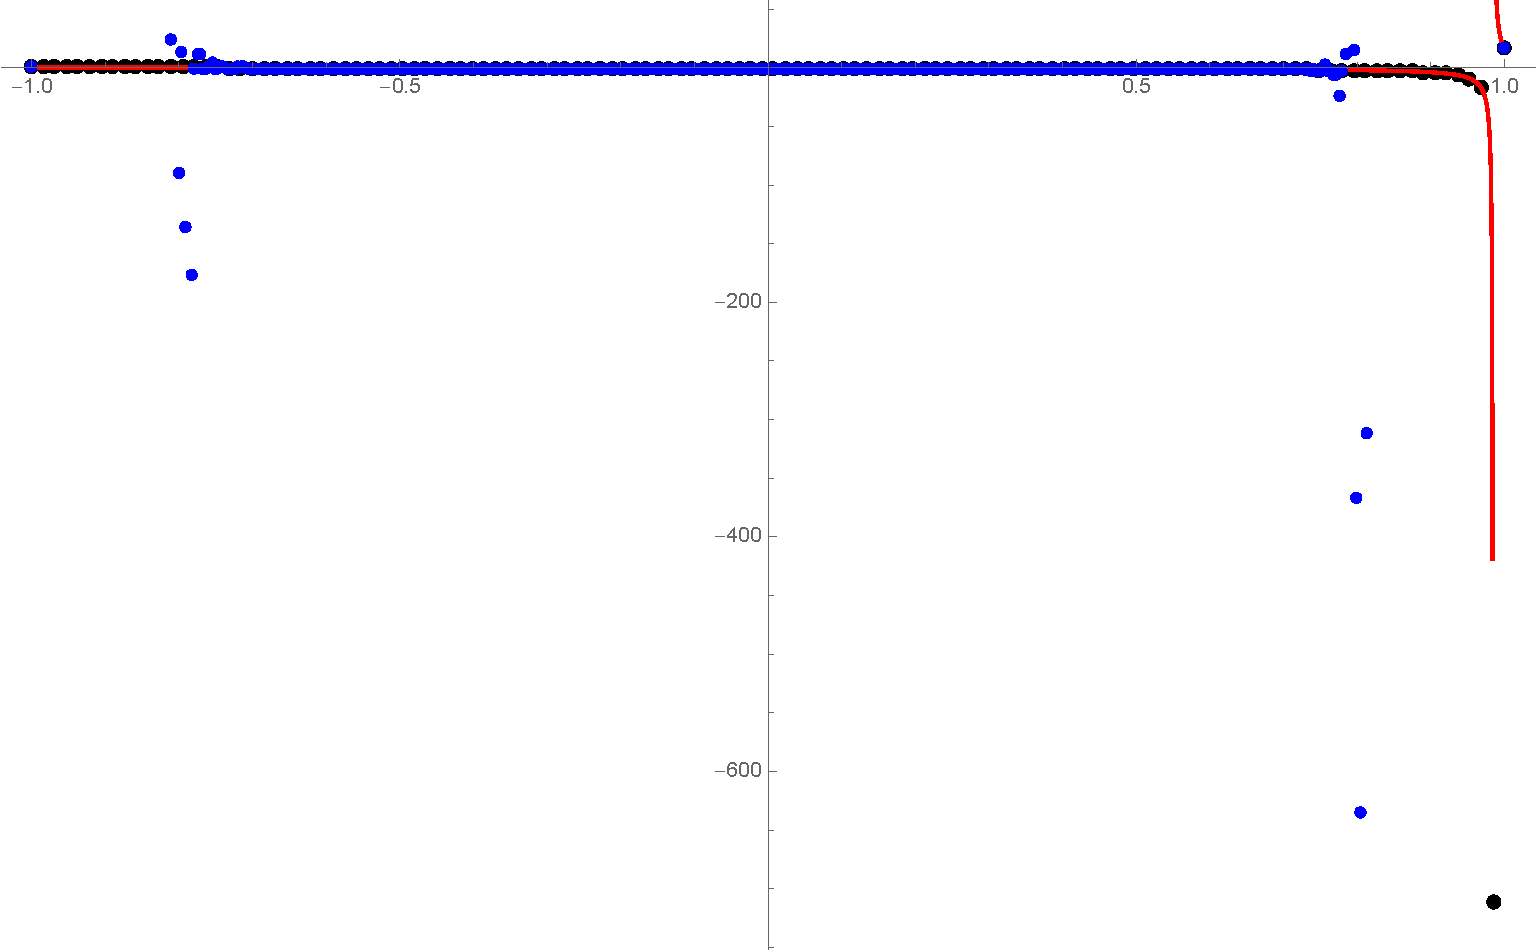
\includegraphics[width=0.8\linewidth]{pic/1/n_128_U.pdf}}
    \caption{Равномерная сетка, $n = 128$, $ \| f(x) - L_n(x)  \|_C = 2.34923e+19 $.}
\end{figure}

\pagebreak


% Чебышевская сетка
\begin{figure}[h]
    \center{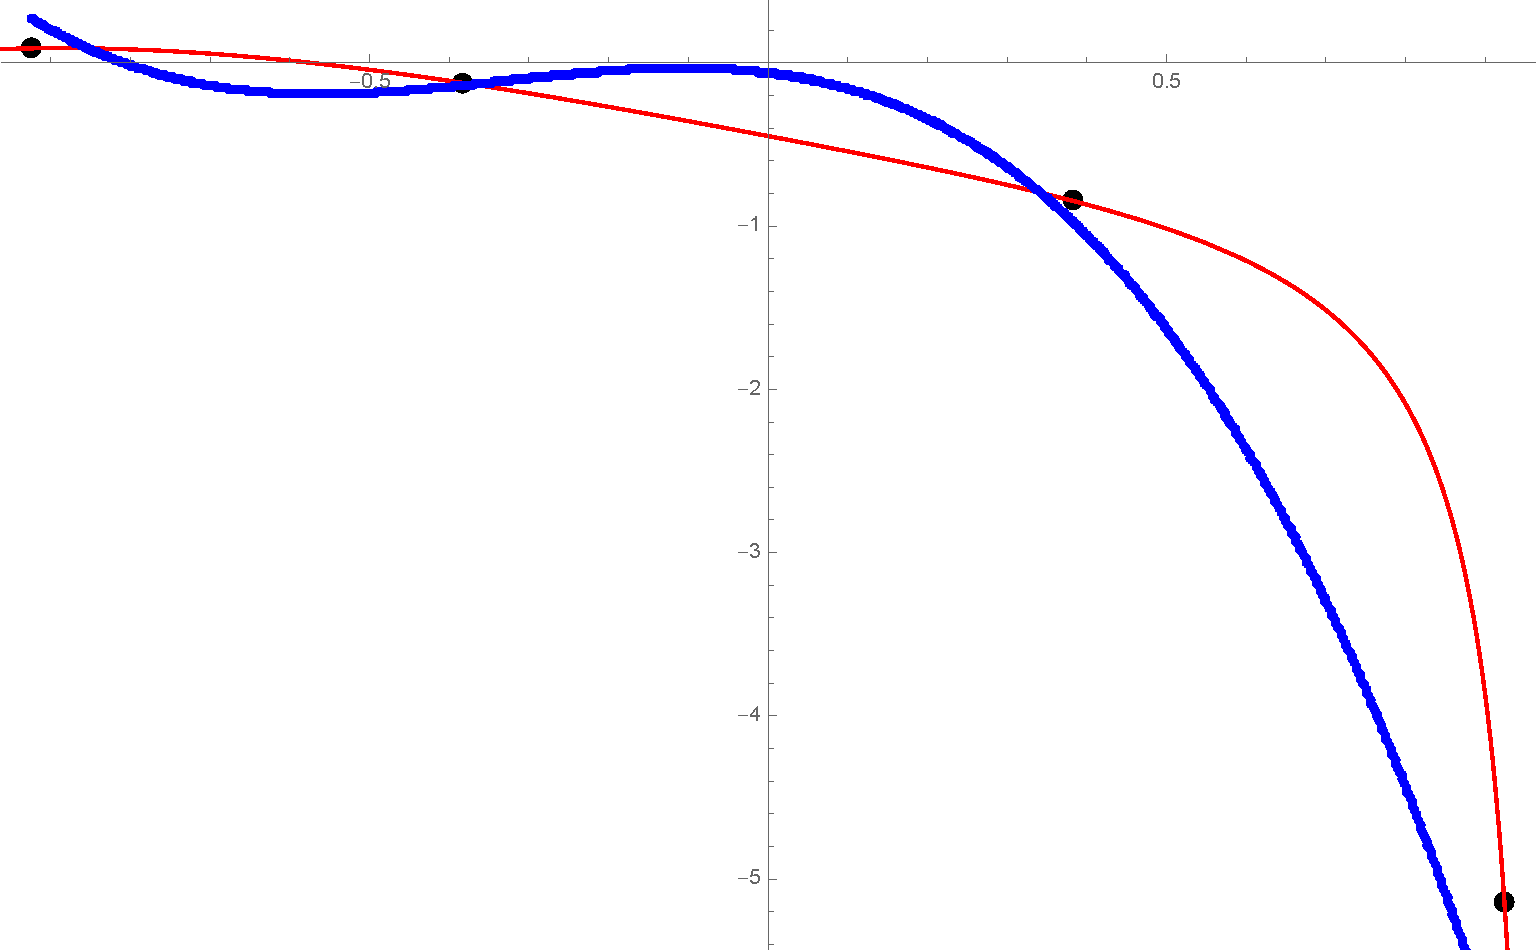
\includegraphics[width=0.8\linewidth]{pic/1/n_4_C.pdf}}
    \caption{Чебышевская сетка, $n = 2$, $ \| f(x) - L_n(x)  \|_C = 2.40999 $.}
\end{figure}

\begin{figure}[h]
    \center{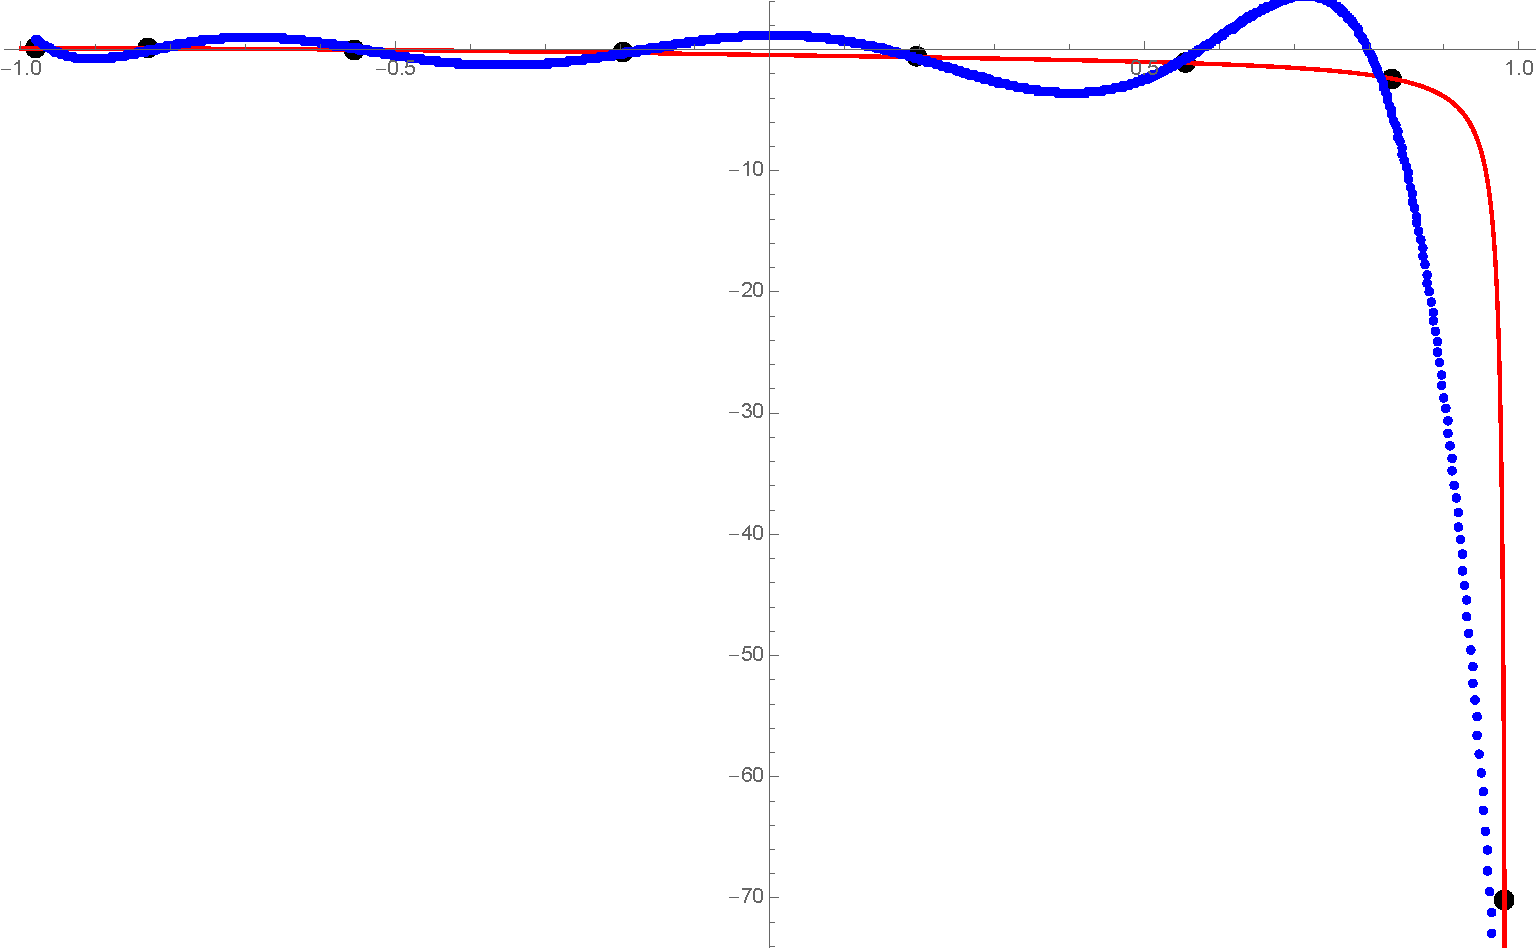
\includegraphics[width=0.8\linewidth]{pic/1/n_8_C.pdf}}
    \caption{Чебышевская сетка, $n = 8$, $ \| f(x) - L_n(x)  \|_C = 57.0232 $.}
\end{figure}

\pagebreak


\begin{figure}[h]
    \center{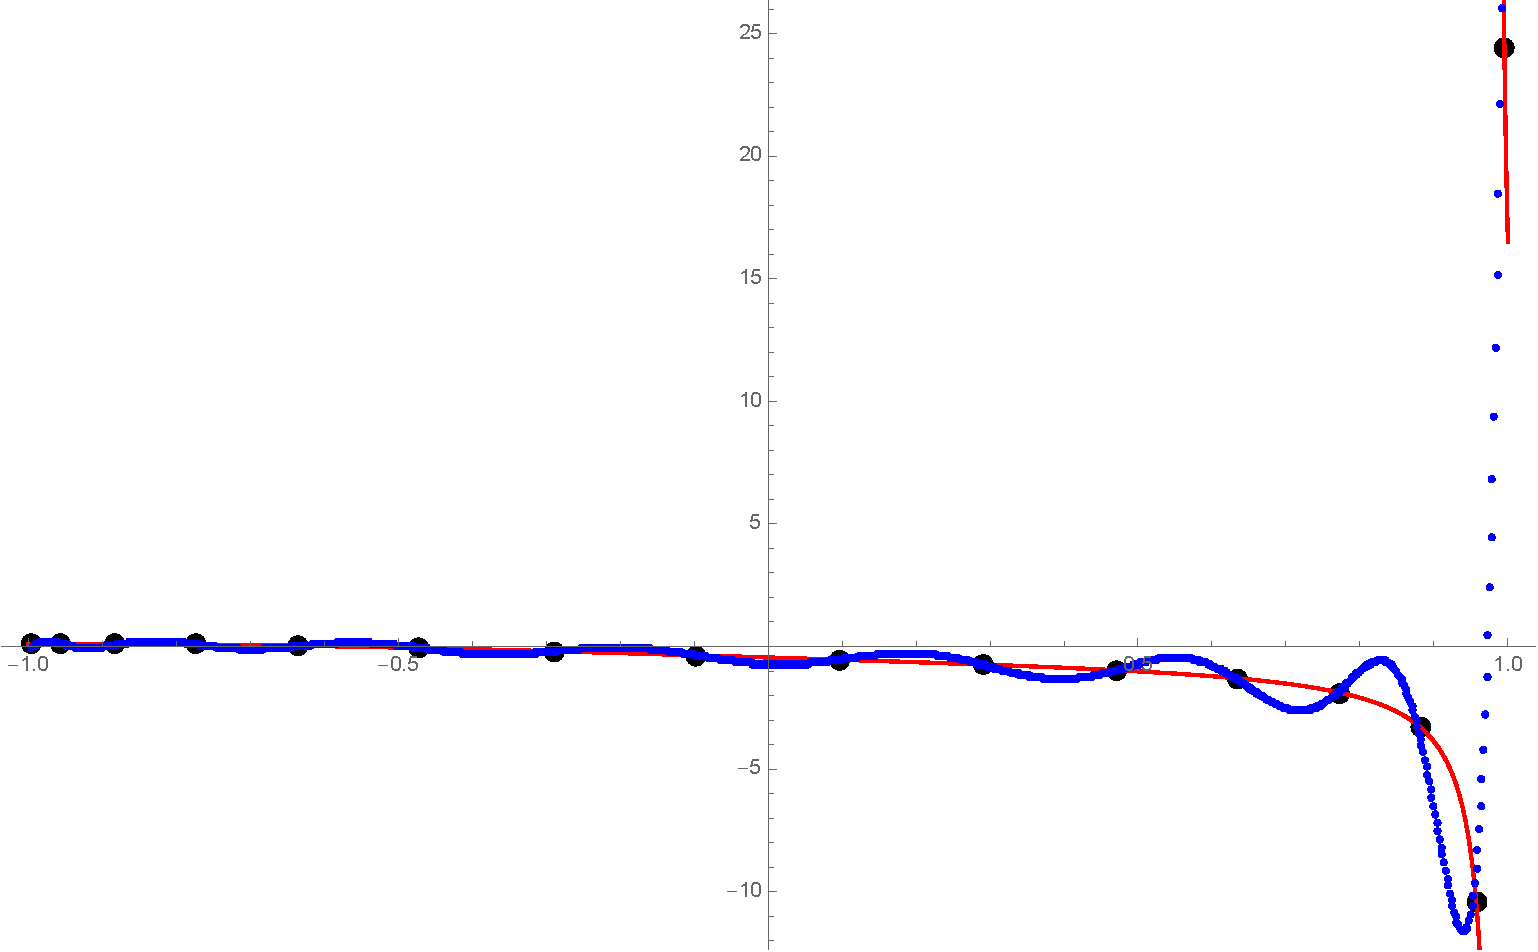
\includegraphics[width=0.8\linewidth]{pic/1/n_16_C.pdf}}
    \caption{Чебышевская сетка, $n = 16$, $ \| f(x) - L_n(x)  \|_C = 441.702 $.}
\end{figure}

\begin{figure}[h]
    \center{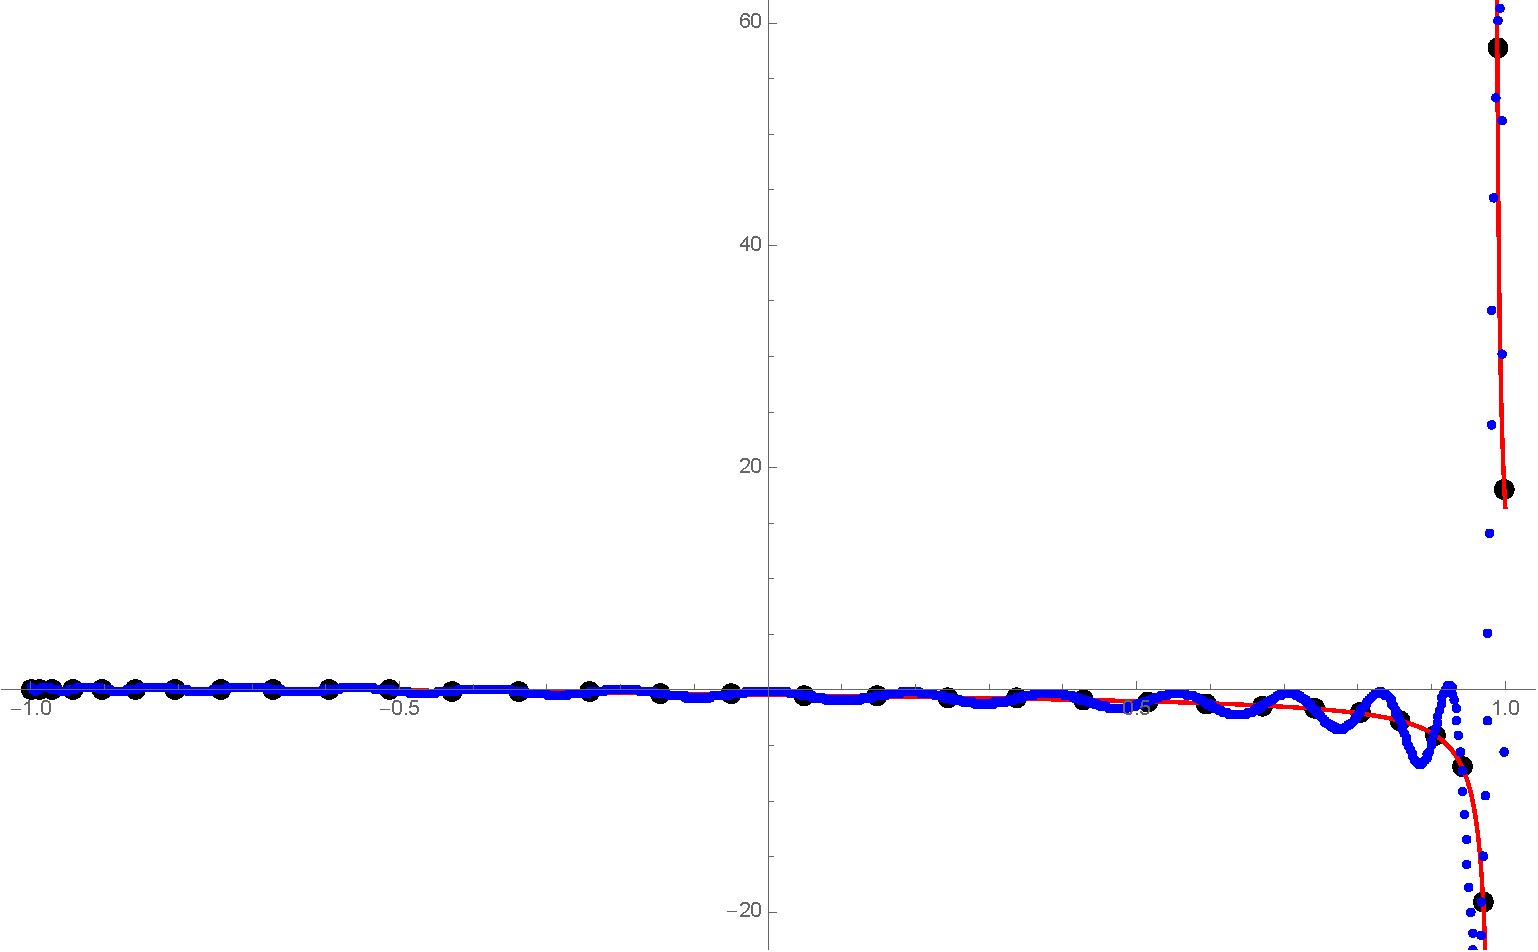
\includegraphics[width=0.8\linewidth]{pic/1/n_32_C.pdf}}
    \caption{Чебышевская сетка, $n = 32$, $ \| f(x) - L_n(x)  \|_C = 1659.45 $.}
\end{figure}

\pagebreak


\begin{figure}[h]
    \center{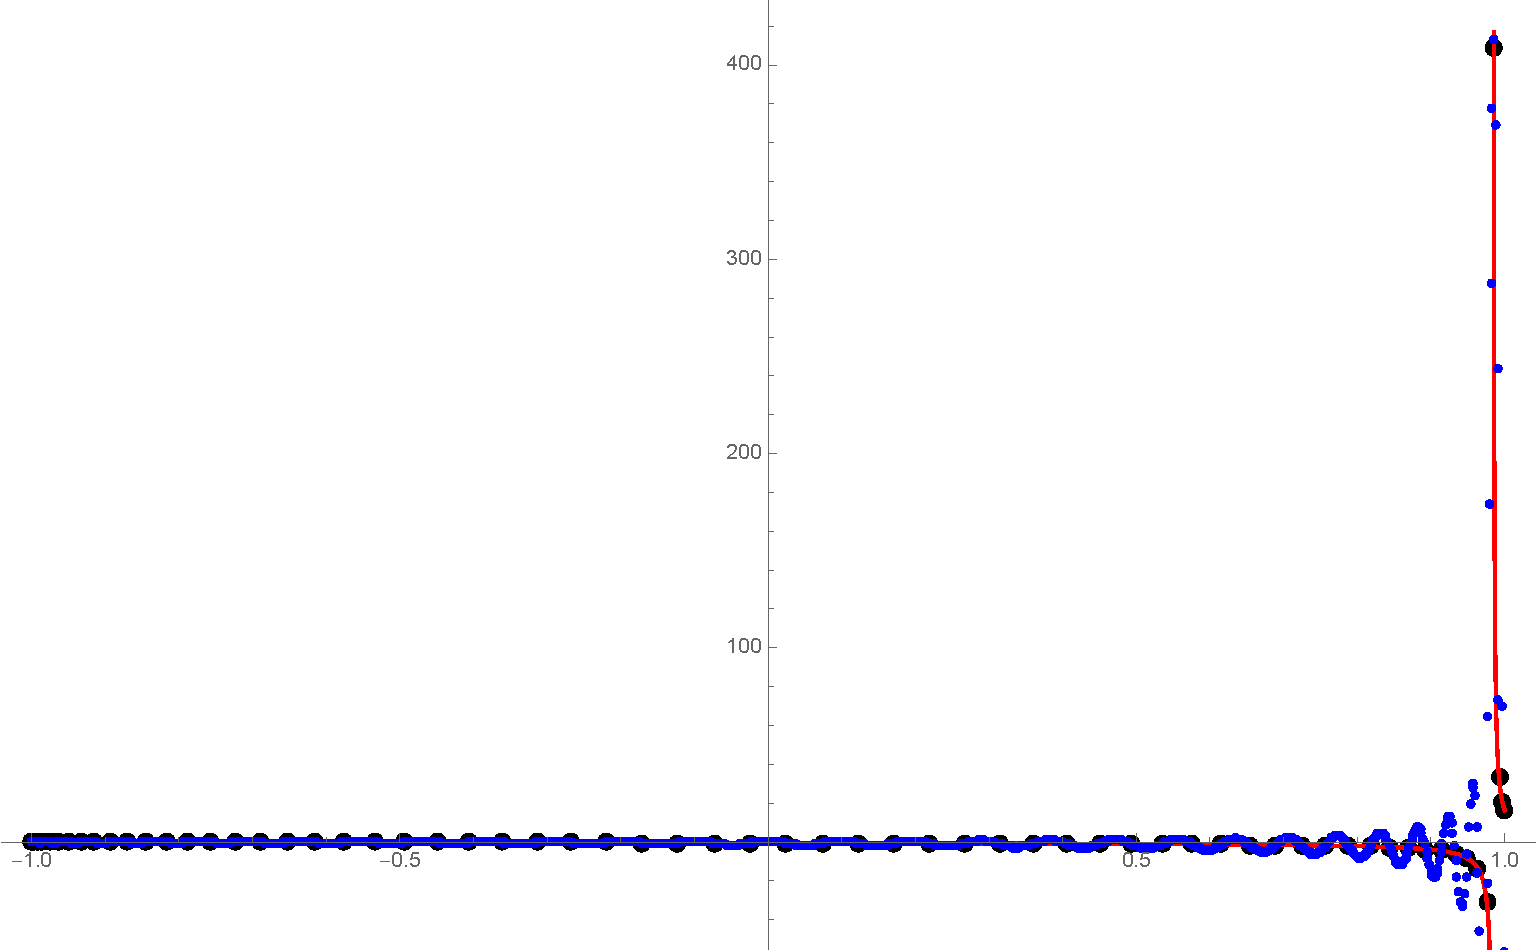
\includegraphics[width=0.8\linewidth]{pic/1/n_64_C.pdf}}
    \caption{Чебышевская сетка, $n = 64$, $ \| f(x) - L_n(x)  \|_C = 567 $.}
\end{figure}

\begin{figure}[h]
    \center{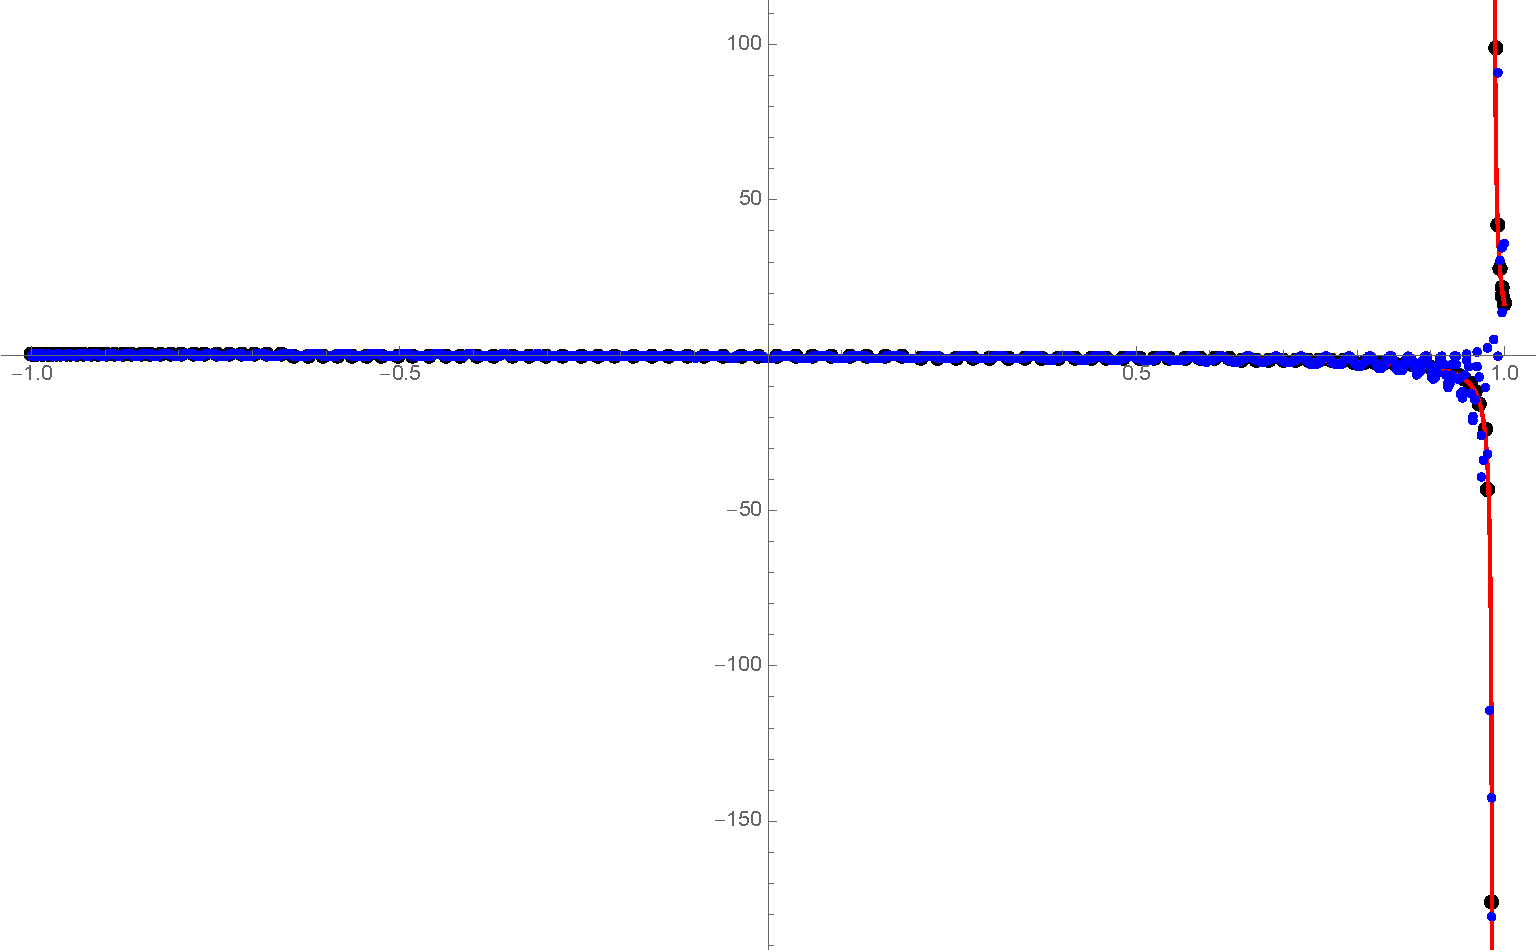
\includegraphics[width=0.8\linewidth]{pic/1/n_128_C.pdf}}
    \caption{Чебышевская сетка, $n = 128$, $ \| f(x) - L_n(x)  \|_C = 351.303 $.}
\end{figure}

\pagebreak

\subsection{Второй пункт}

\begin{figure}[h]
    \center{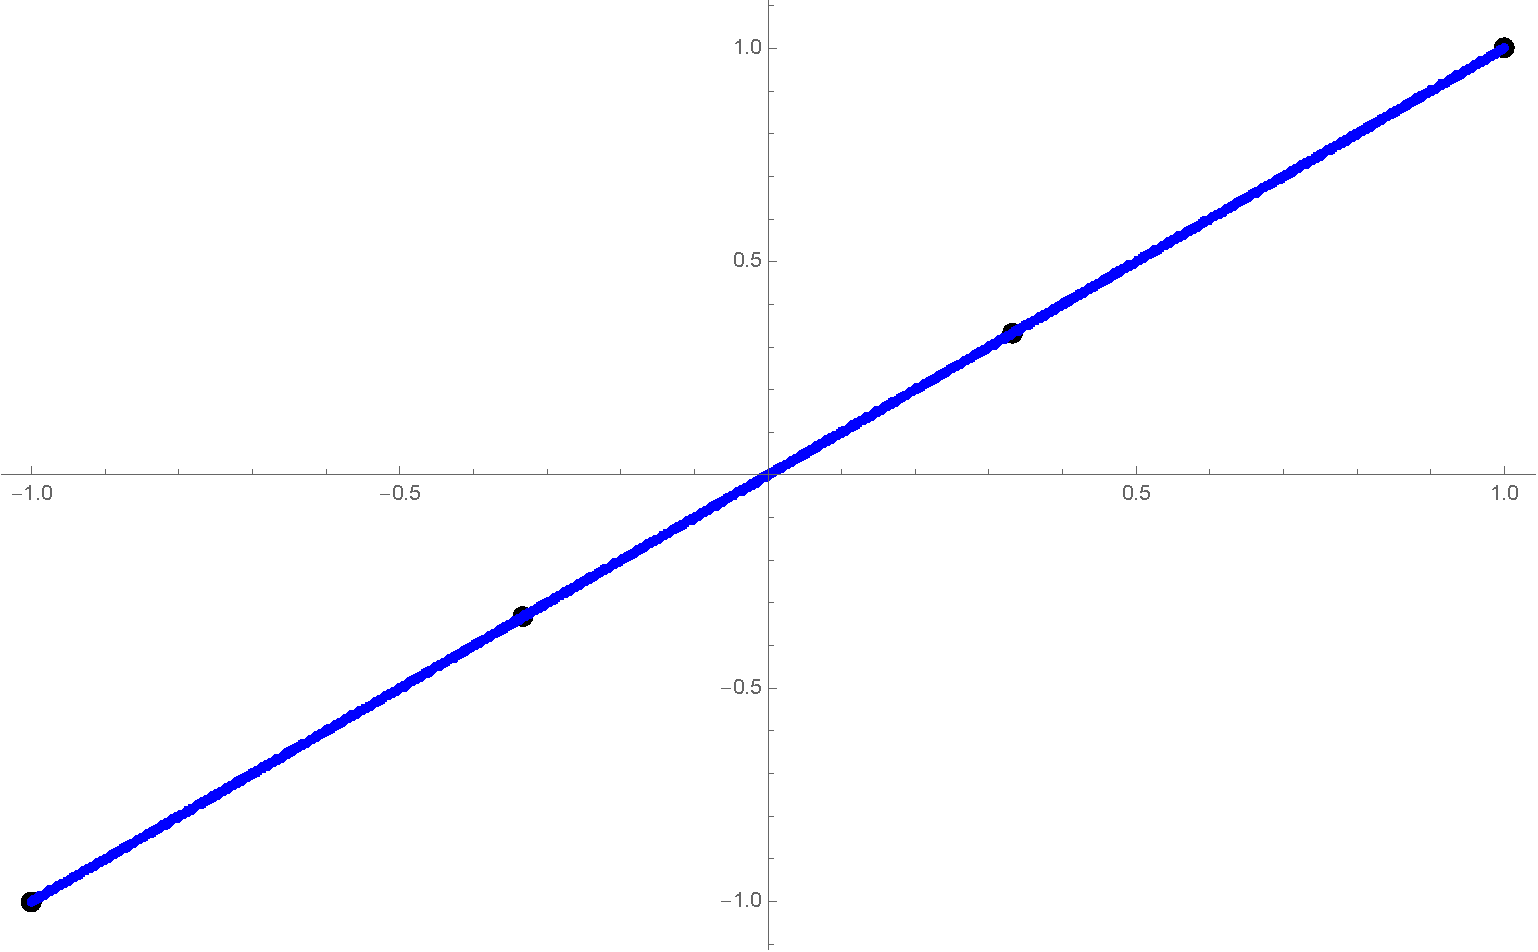
\includegraphics[width=0.8\linewidth]{pic/2/n_4_U.pdf}}
    \caption{Равномерная сетка, $n = 4$, $ \| f(x) - L_n(x)  \|_C = 0.00200401 $.}
\end{figure}

\begin{figure}[h]
    \center{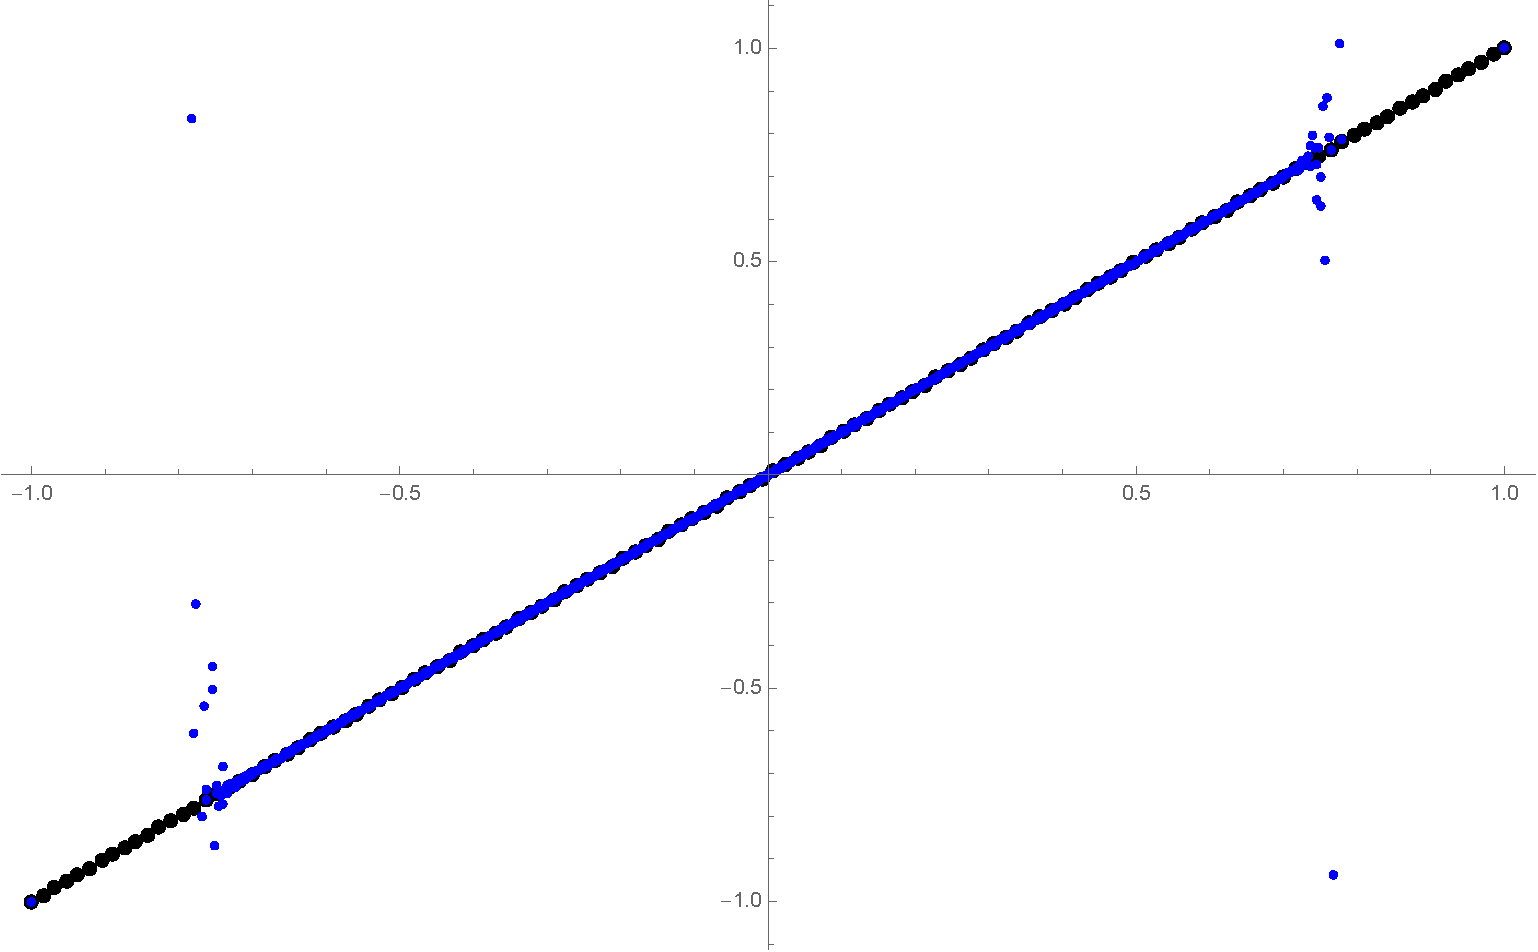
\includegraphics[width=0.8\linewidth]{pic/2/n_128_U.pdf}}
    \caption{Равномерная сетка, $n = 128$, $ \| f(x) - L_n(x)  \|_C = 2.84368e+18 $.}
\end{figure}

\pagebreak


\begin{figure}[h]
    \center{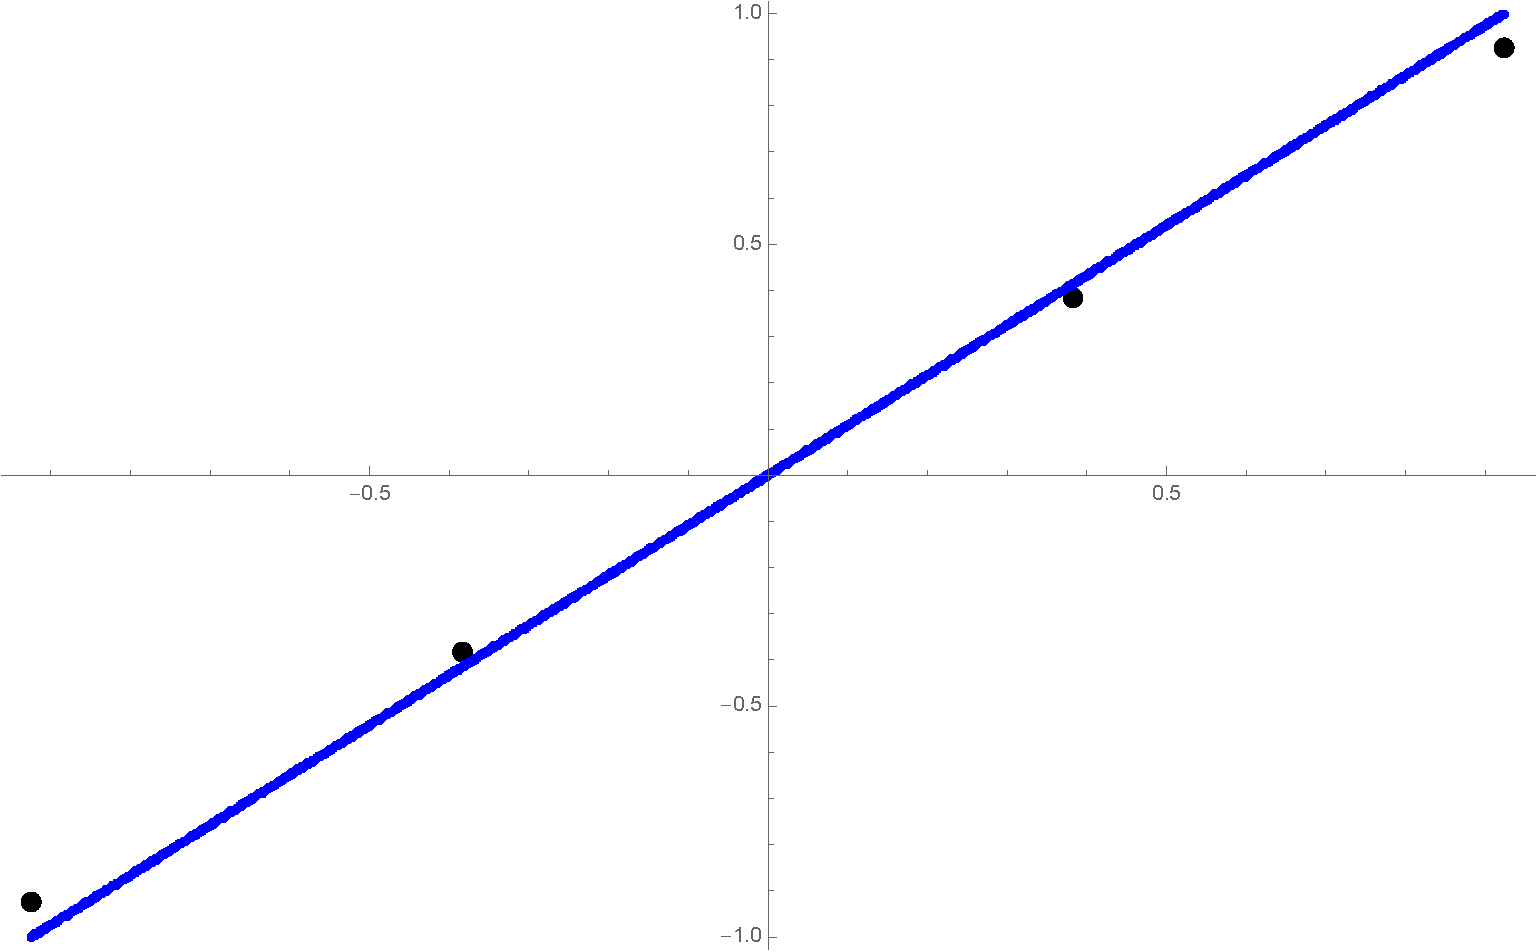
\includegraphics[width=0.8\linewidth]{pic/2/n_4_C.pdf}}
    \caption{Чебышевская сетка, $n = 4$, $ \| f(x) - L_n(x)  \|_C = 0.0761205 $.}
\end{figure}

\begin{figure}[h]
    \center{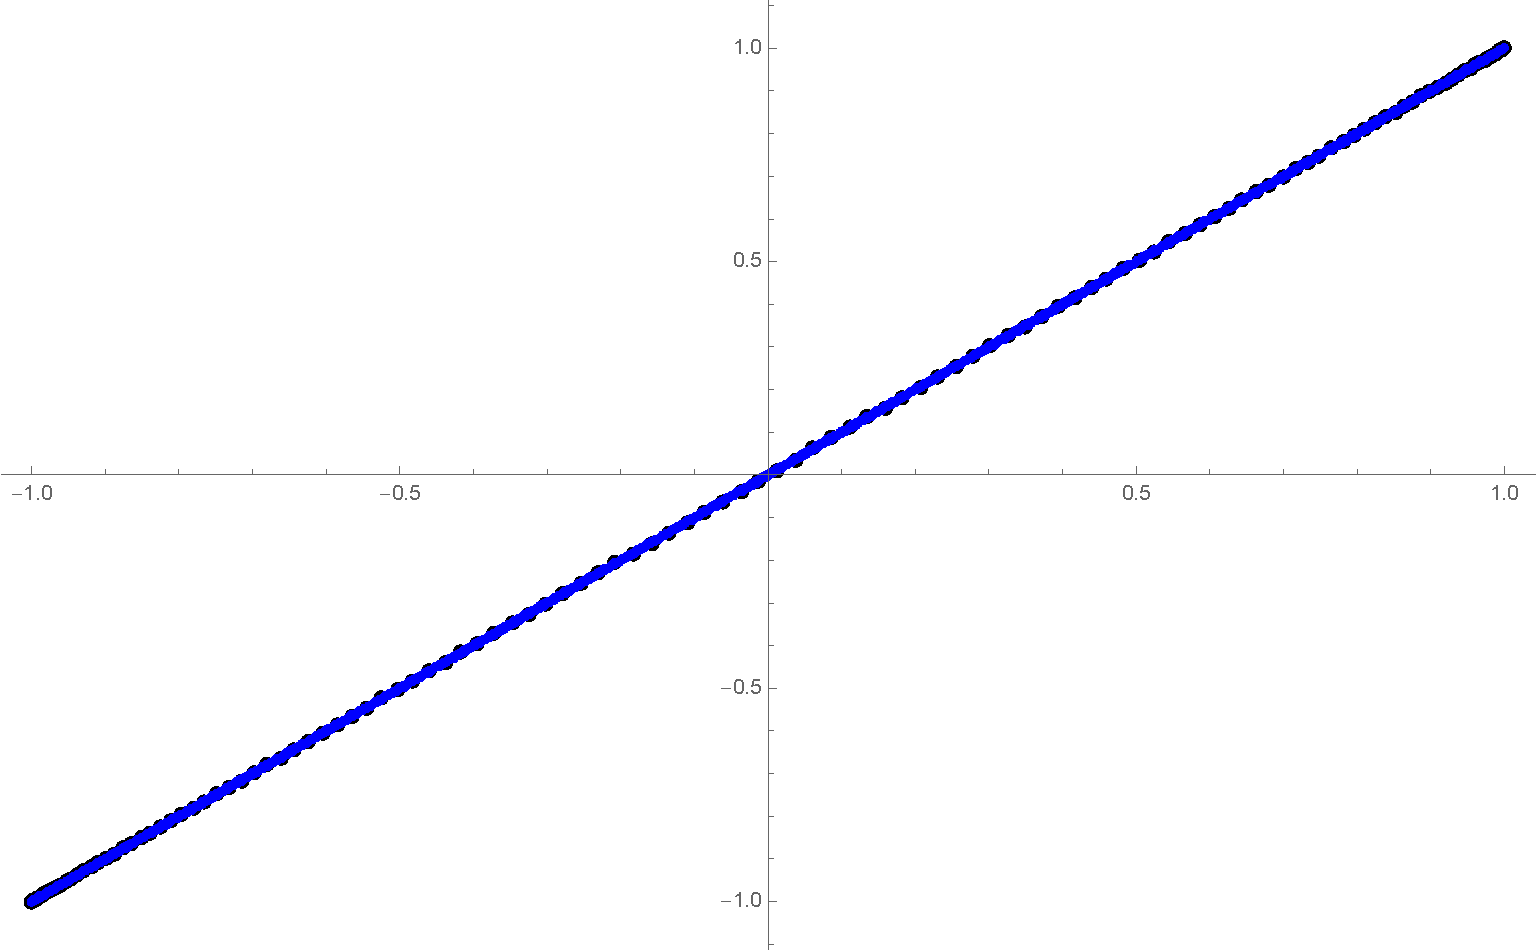
\includegraphics[width=0.8\linewidth]{pic/2/n_128_C.pdf}}
    \caption{Чебышевская сетка, $n = 128$, $ \| f(x) - L_n(x)  \|_C = 0.00192856 $.}
\end{figure}

\pagebreak



\subsection{Третий пункт}

\begin{figure}[h]
    \center{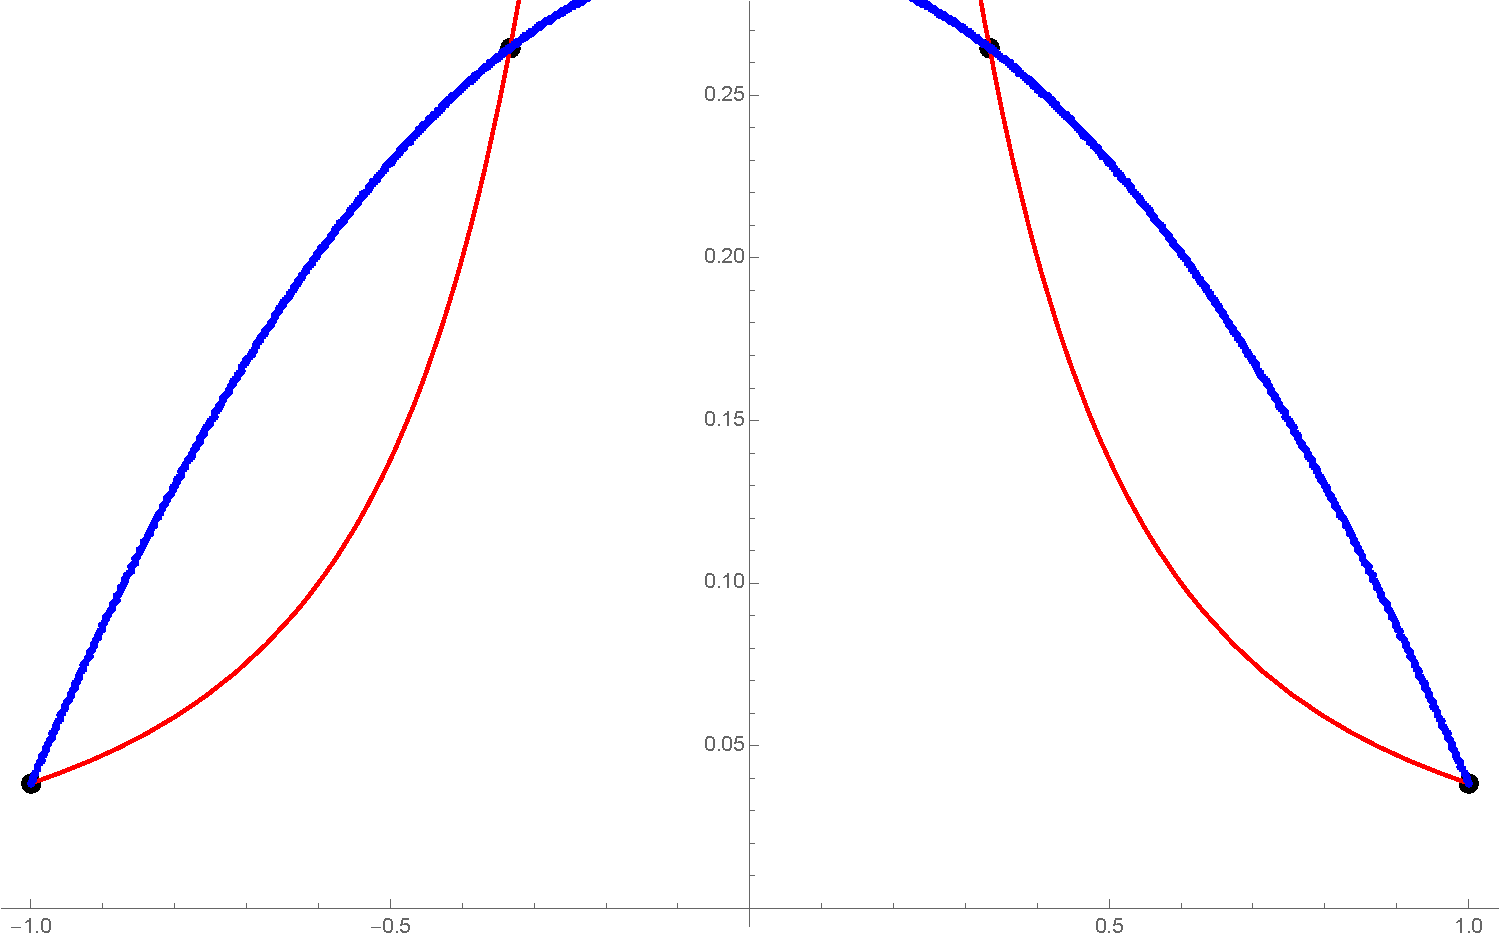
\includegraphics[width=0.8\linewidth]{pic/3/n_4_U.pdf}}
    \caption{Равномерная сетка, $n = 4$, $ \| f(x) - L_n(x)  \|_C = 0.707014 $.}
\end{figure}

\begin{figure}[h]
    \center{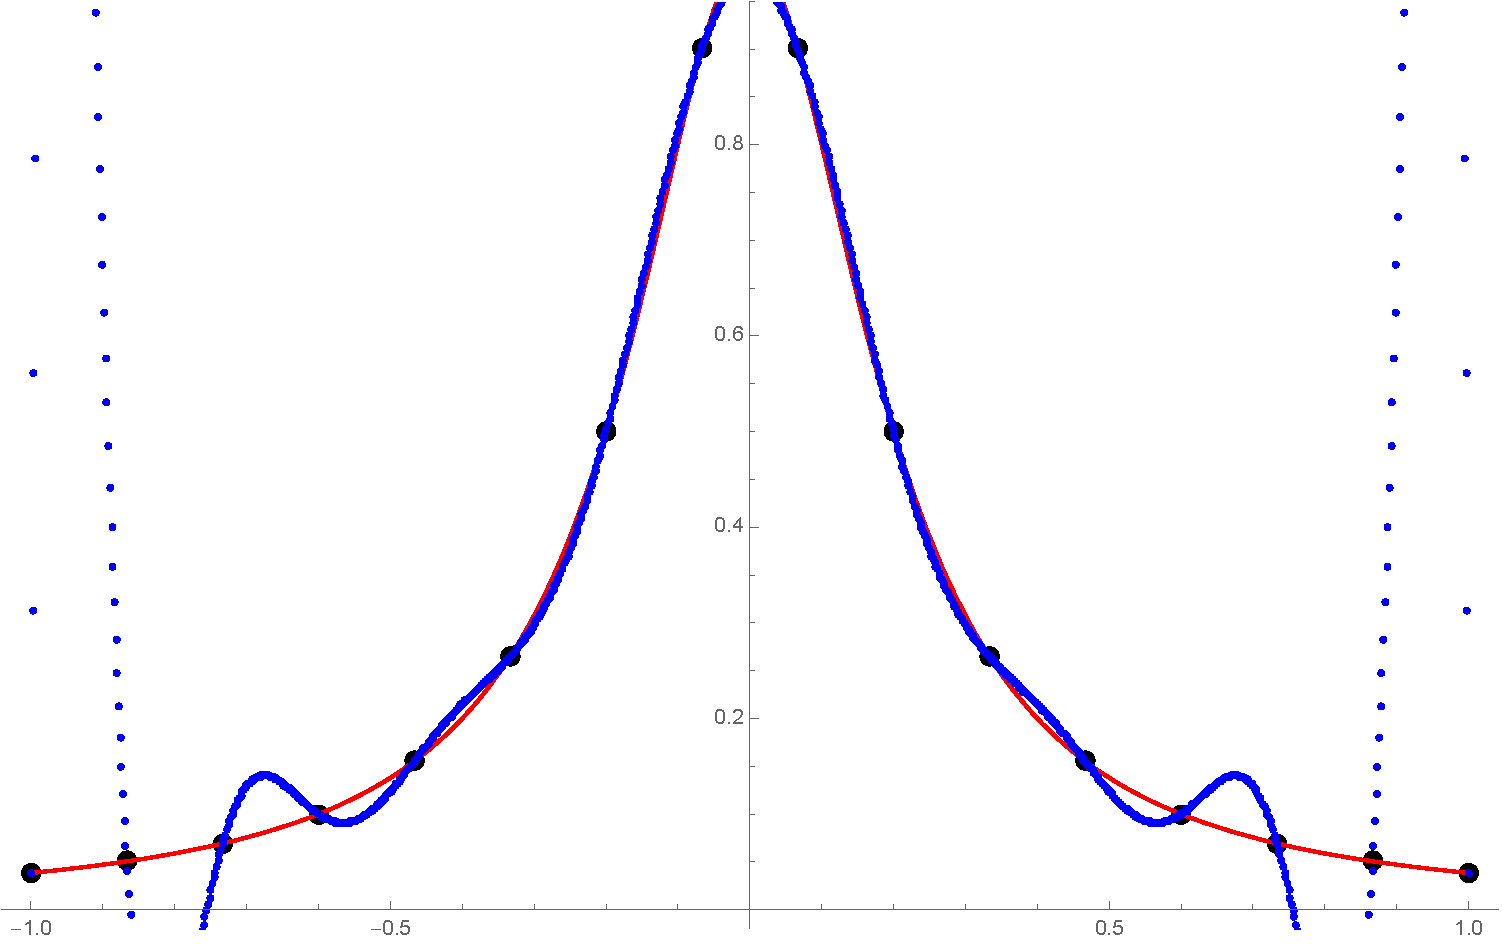
\includegraphics[width=0.8\linewidth]{pic/3/n_16_U.pdf}}
    \caption{Равномерная сетка, $n = 16$, $ \| f(x) - L_n(x)  \|_C = 2.10702 $.}
\end{figure}

\pagebreak


\begin{figure}[h]
    \center{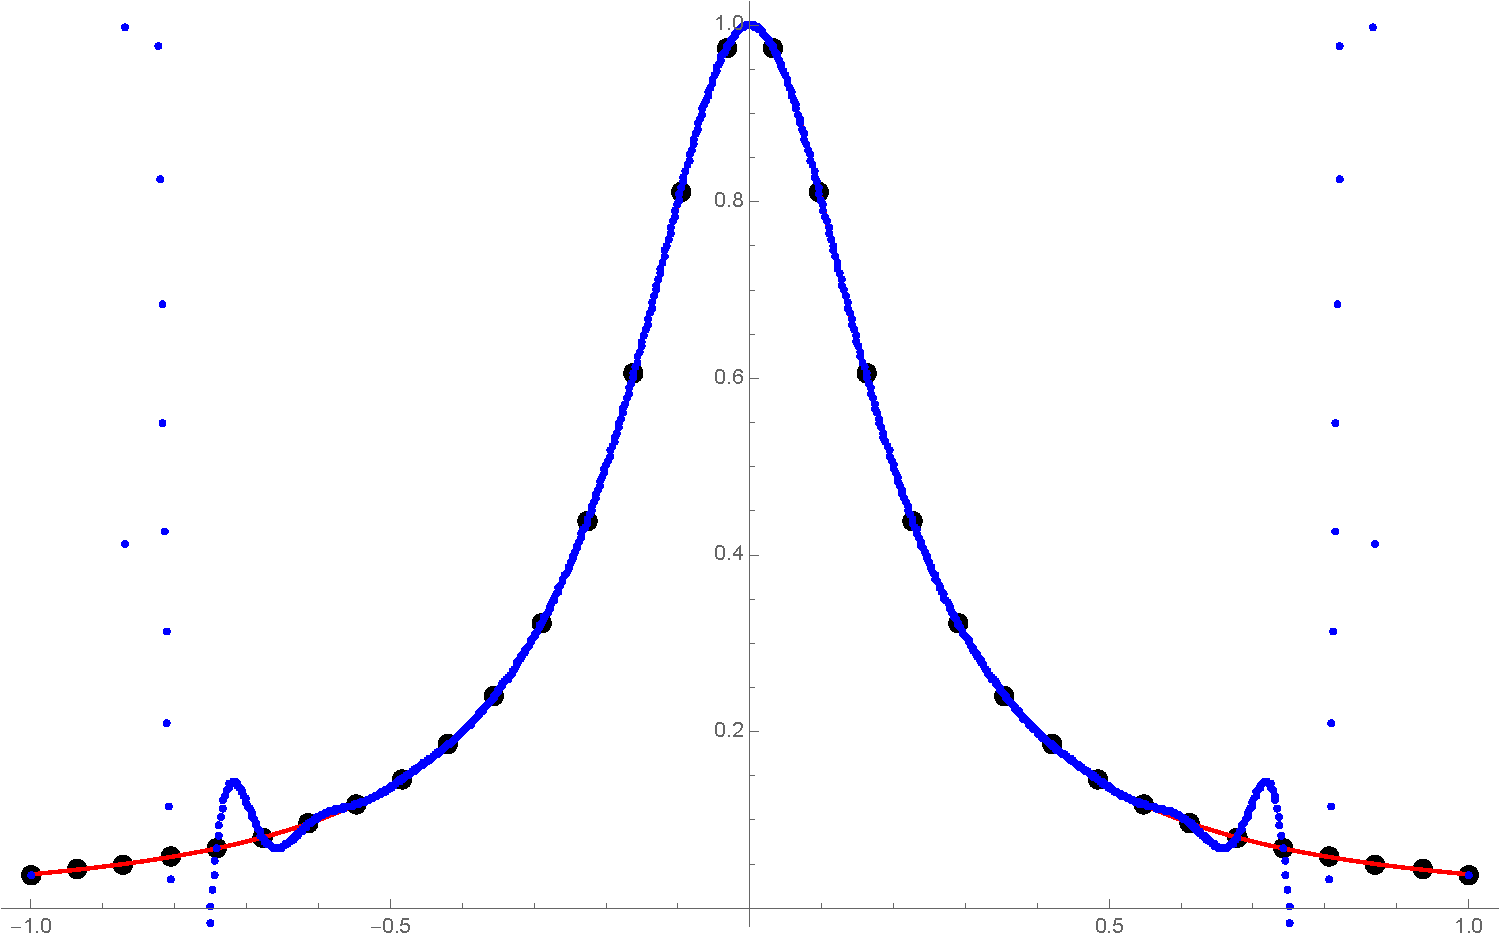
\includegraphics[width=0.8\linewidth]{pic/3/n_32_U.pdf}}
    \caption{Равномерная сетка, $n = 32$, $ \| f(x) - L_n(x)  \|_C = 704.076 $.}
\end{figure}

\begin{figure}[h]
    \center{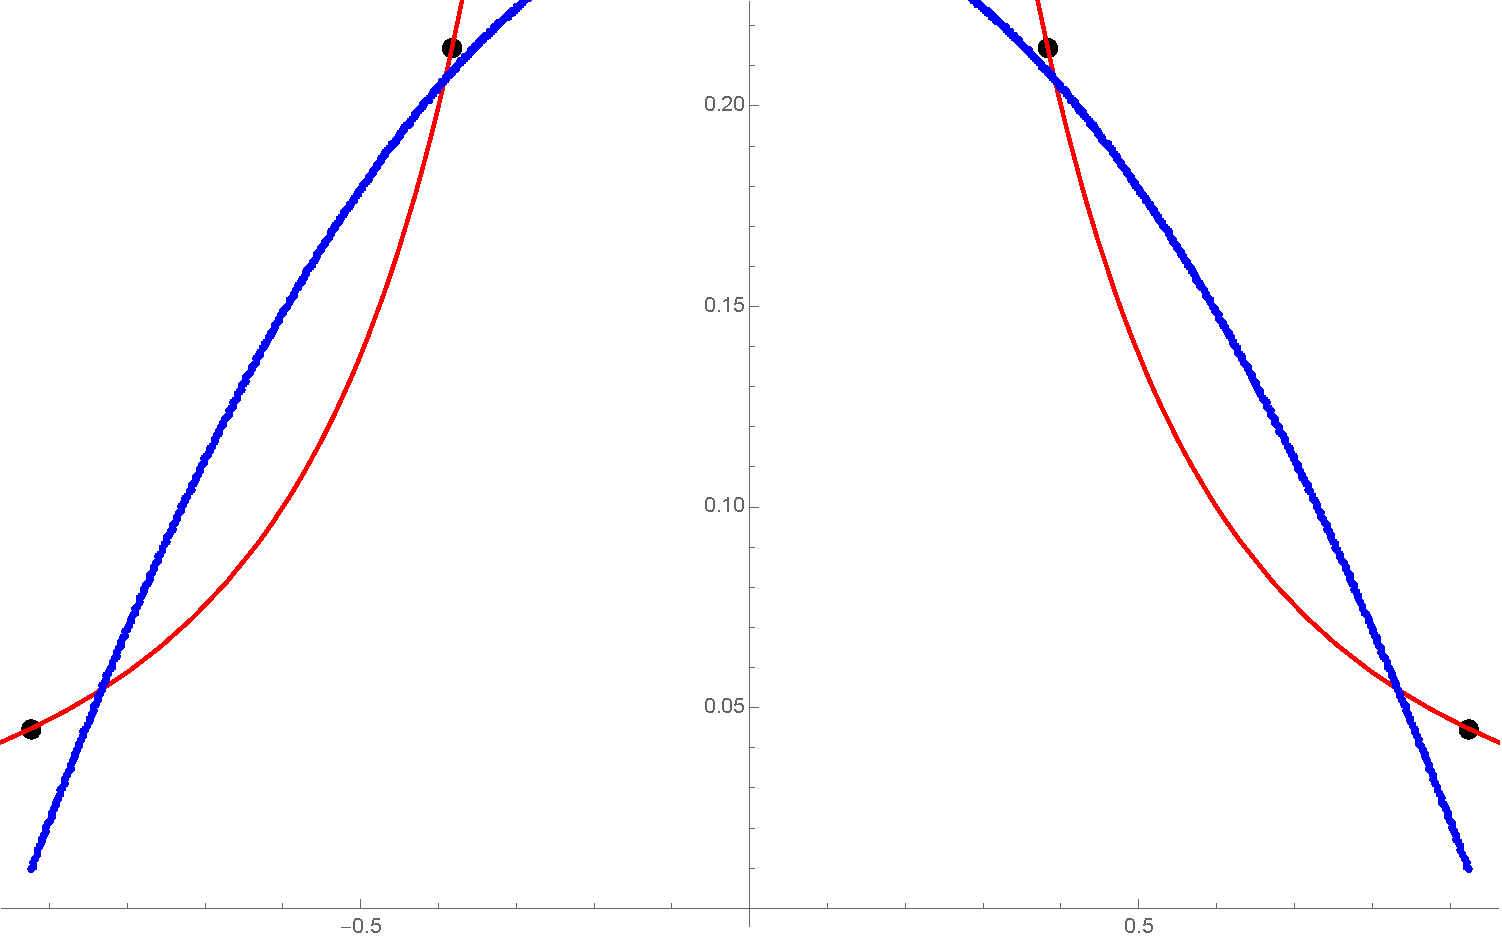
\includegraphics[width=0.8\linewidth]{pic/3/n_4_C.pdf}}
    \caption{Чебышевская сетка, $n = 4$, $ \| f(x) - L_n(x)  \|_C = 0.7503 $.}
\end{figure}

\pagebreak


\begin{figure}[h]
    \center{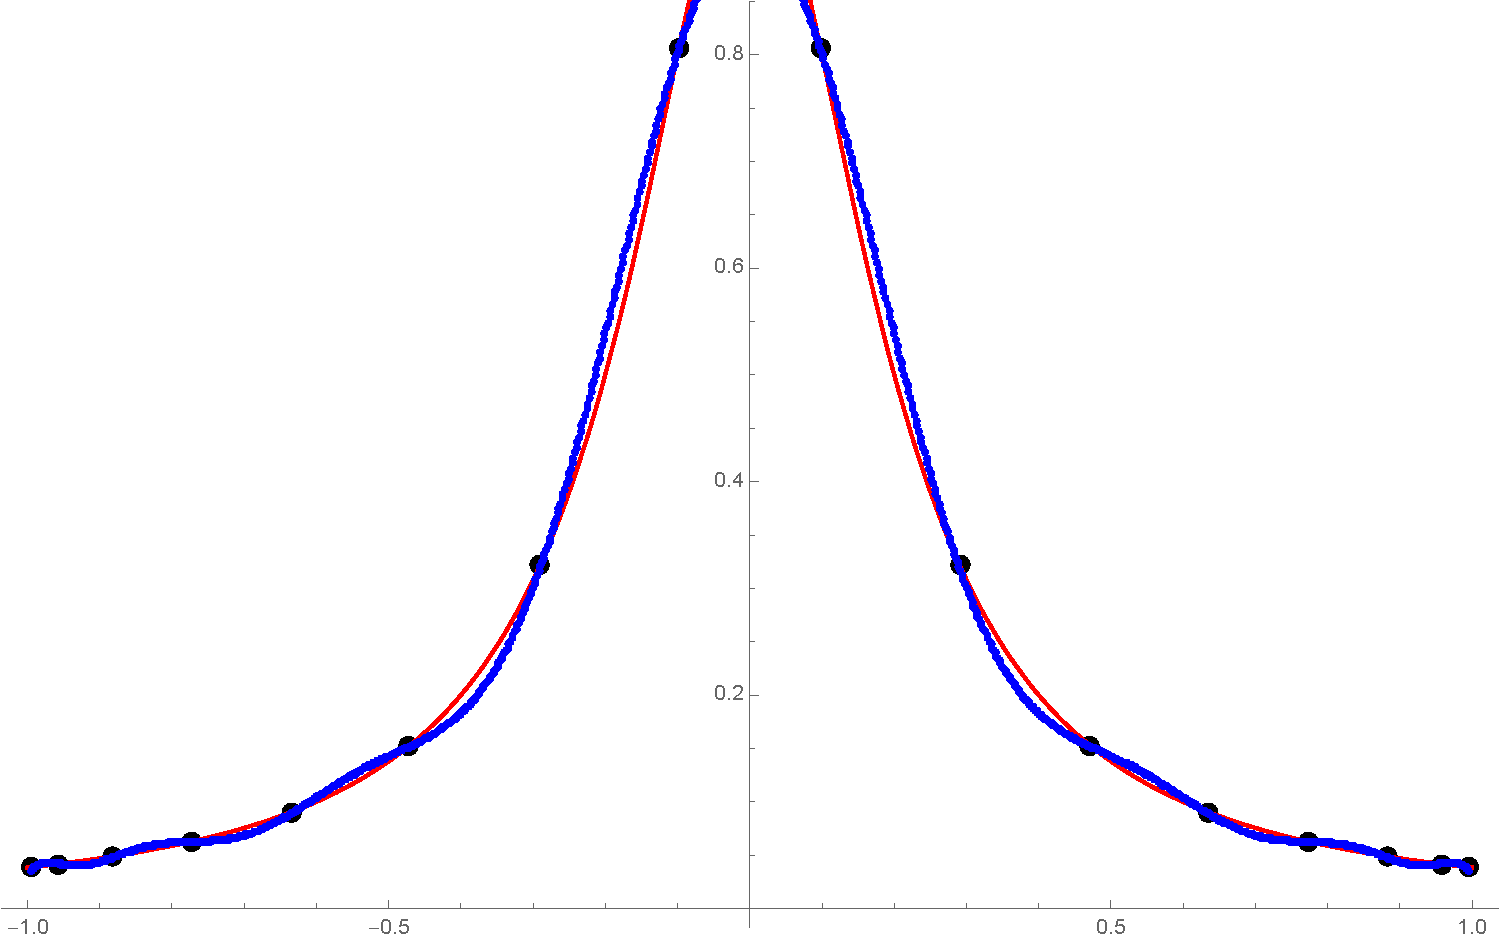
\includegraphics[width=0.8\linewidth]{pic/3/n_16_C.pdf}}
    \caption{Чебышевская сетка, $n = 16$, $ \| f(x) - L_n(x)  \|_C = 0.0831194 $.}
\end{figure}

\begin{figure}[h]
    \center{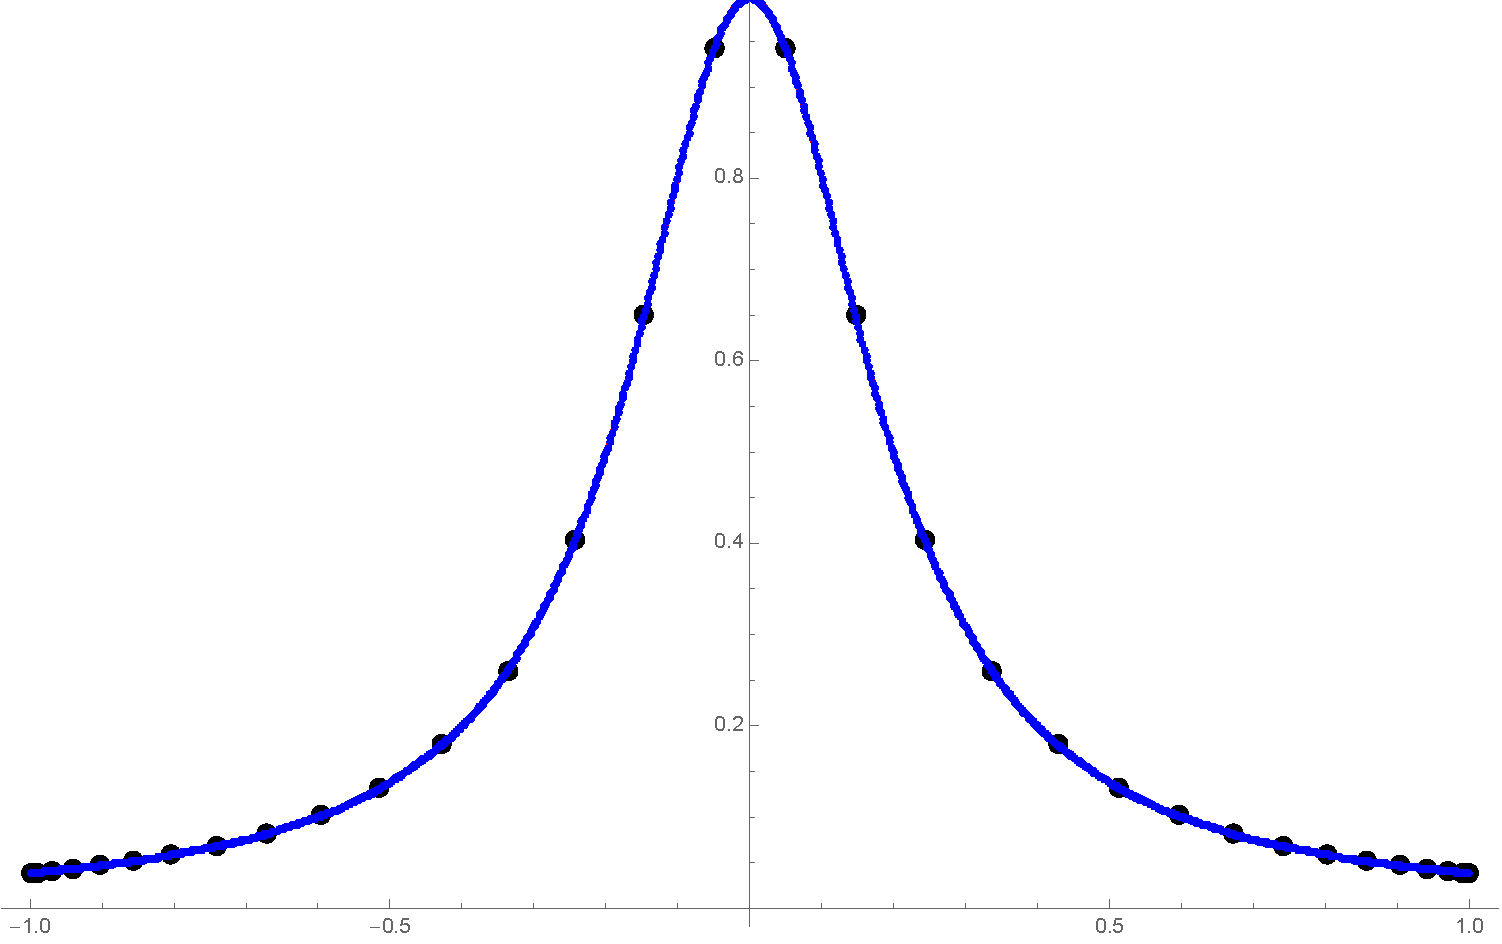
\includegraphics[width=0.8\linewidth]{pic/3/n_32_C.pdf}}
    \caption{Чебышевская сетка, $n = 32$, $ \| f(x) - L_n(x)  \|_C = 0.0059259 $.}
\end{figure}

\pagebreak


\subsection{Четвертый пункт}

\begin{figure}[h]
    \center{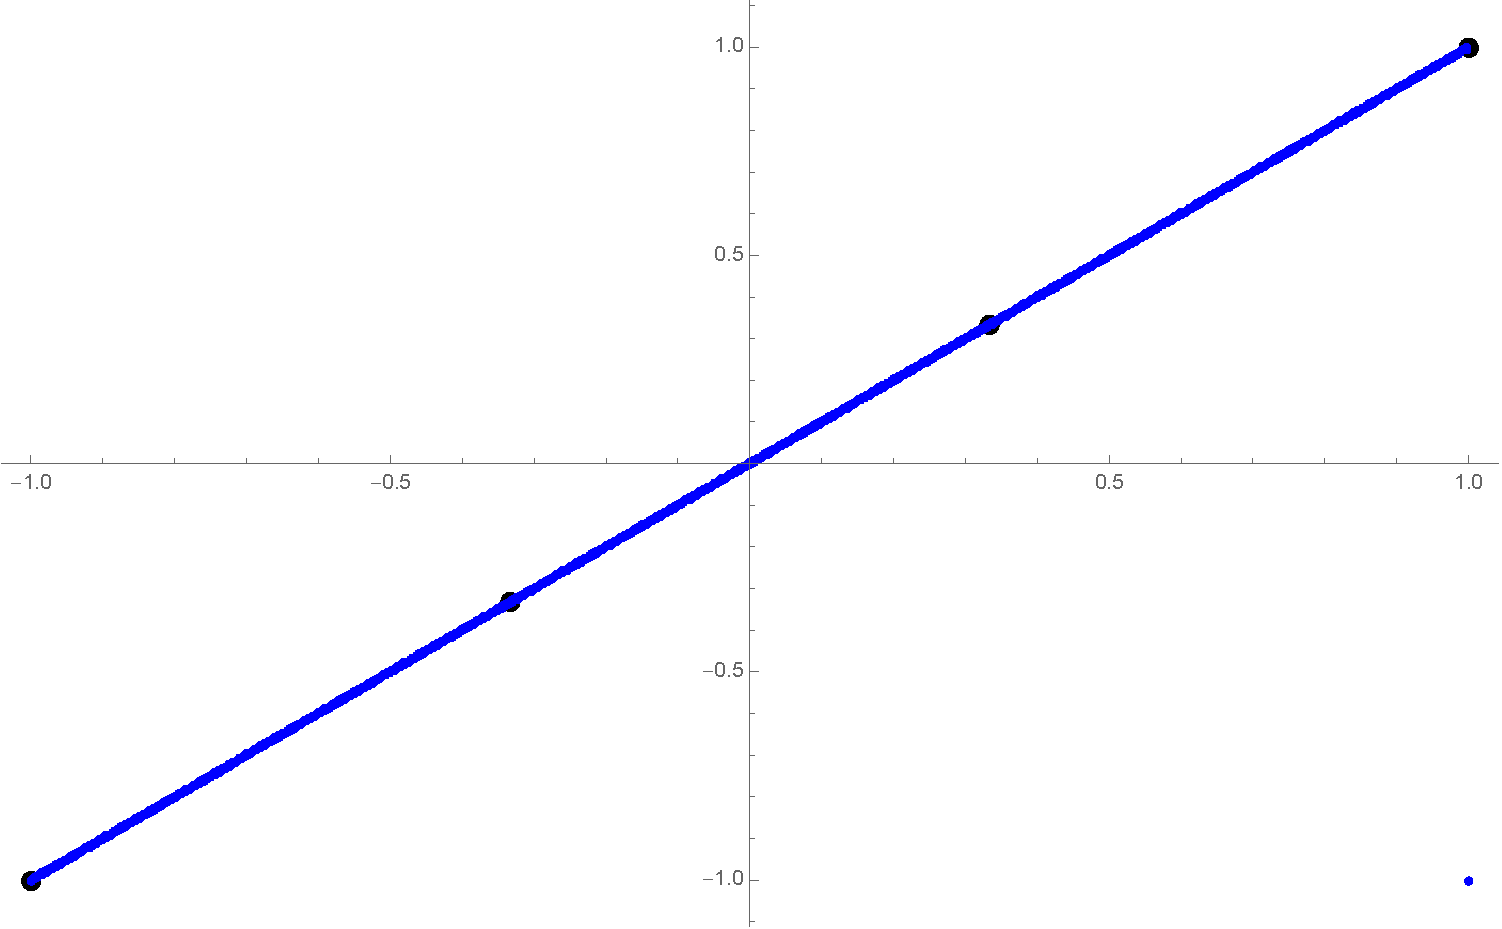
\includegraphics[width=0.8\linewidth]{pic/4/f_n_4_U.pdf}}
    \caption{Равномерная сетка, $f(x) = x$, $n = 4$.}
\end{figure}

\begin{figure}[h]
    \center{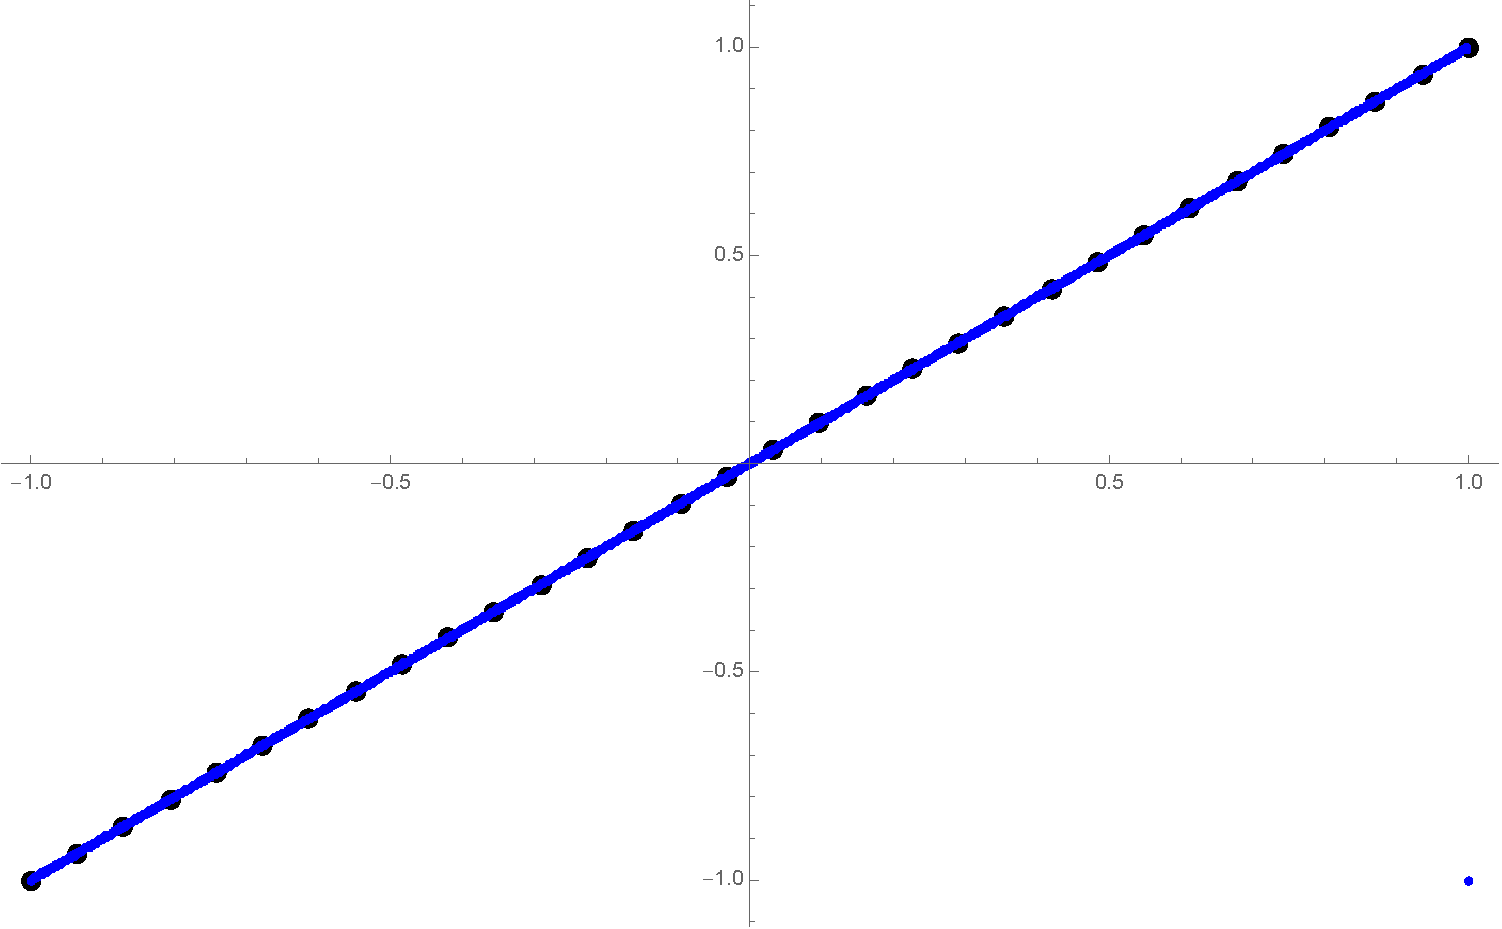
\includegraphics[width=0.8\linewidth]{pic/4/f_n_32_U.pdf}}
    \caption{Равномерная сетка, $f(x) = x$, $n = 32$.}
\end{figure}

\pagebreak


\begin{figure}[h]
    \center{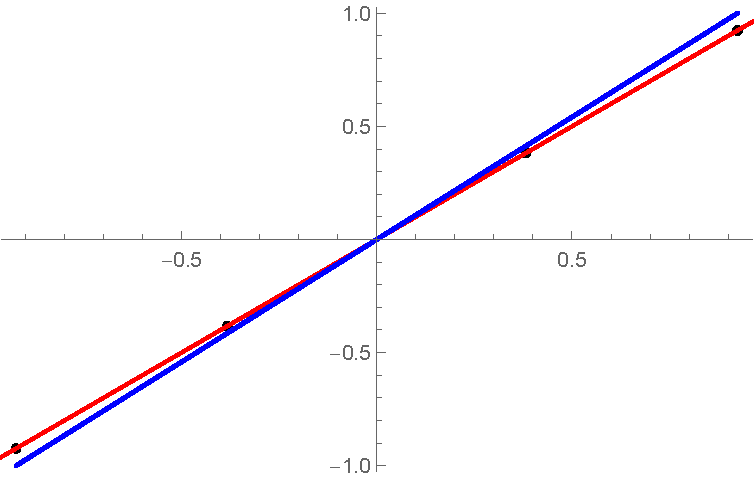
\includegraphics[width=0.8\linewidth]{pic/4/f_n_4_C.pdf}}
    \caption{Чебышевская сетка, $f(x) = x$, $n = 4$.}
\end{figure}

\begin{figure}[h]
    \center{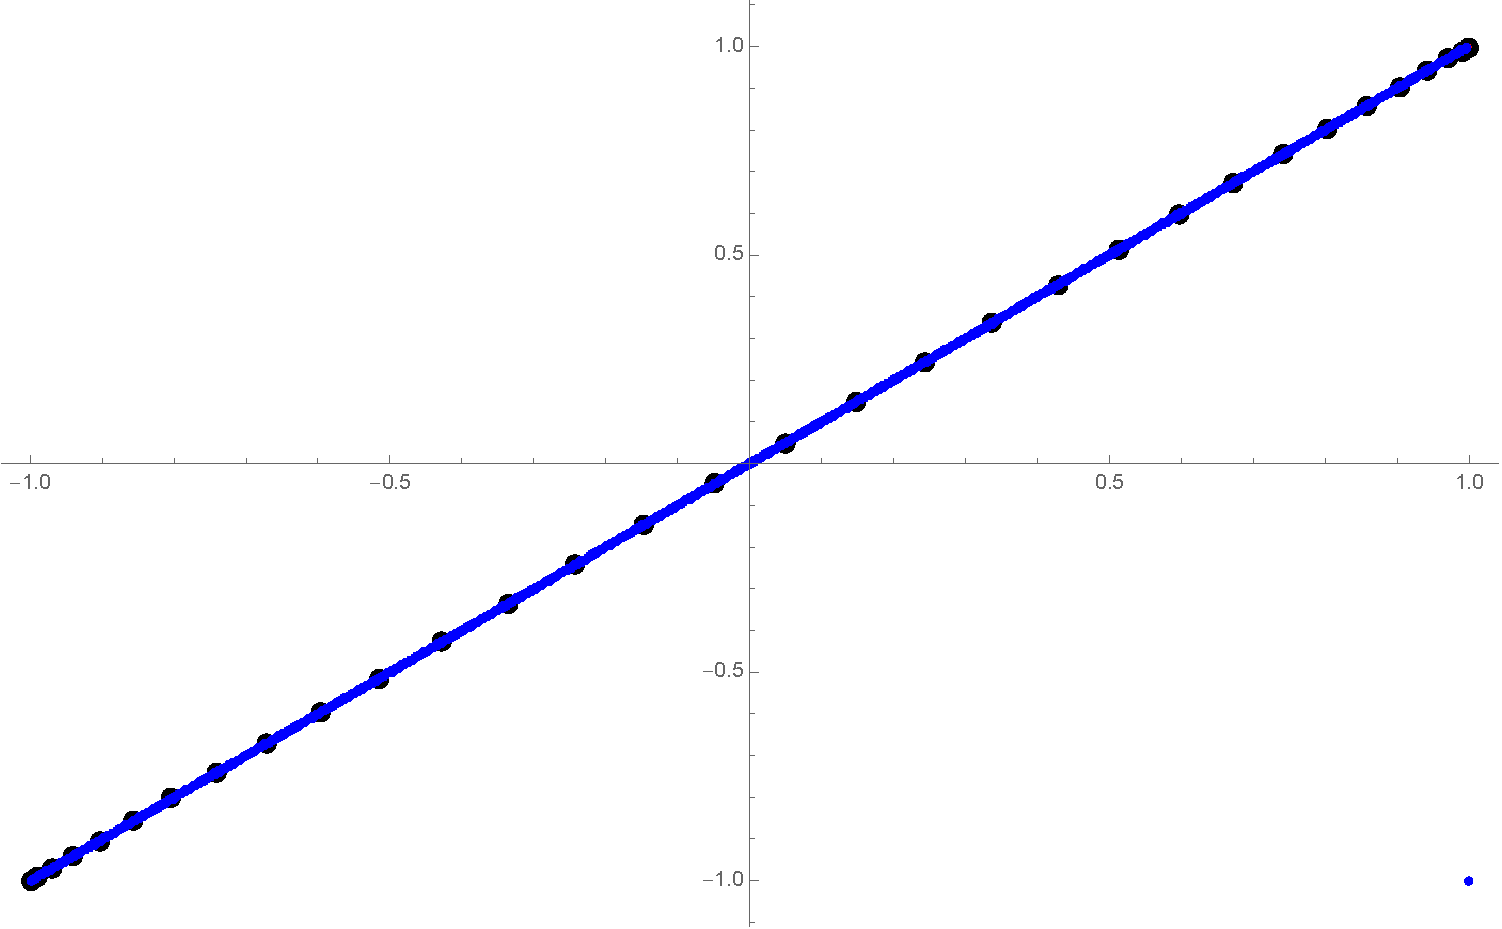
\includegraphics[width=0.8\linewidth]{pic/4/f_n_32_C.pdf}}
    \caption{Чебышевская сетка, $f(x) = x$, $n = 32$.}
\end{figure}

\pagebreak


\begin{figure}[h]
    \center{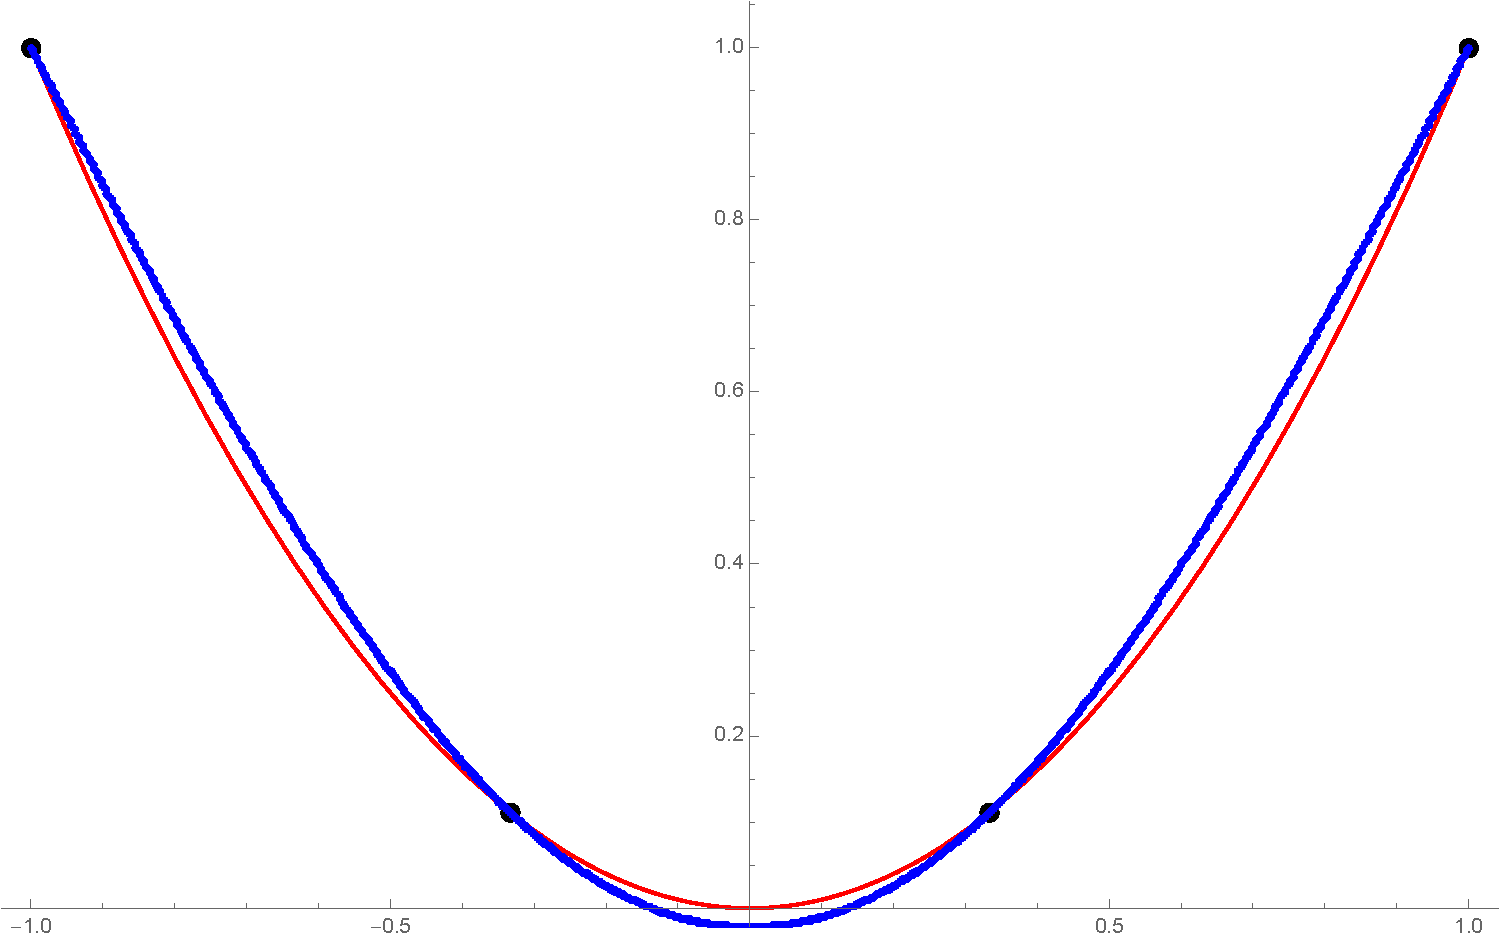
\includegraphics[width=0.8\linewidth]{pic/4/g_n_4_U.pdf}}
    \caption{Равномерная сетка, $g(x) = x^2$, $n = 4$.}
\end{figure}

\begin{figure}[h]
    \center{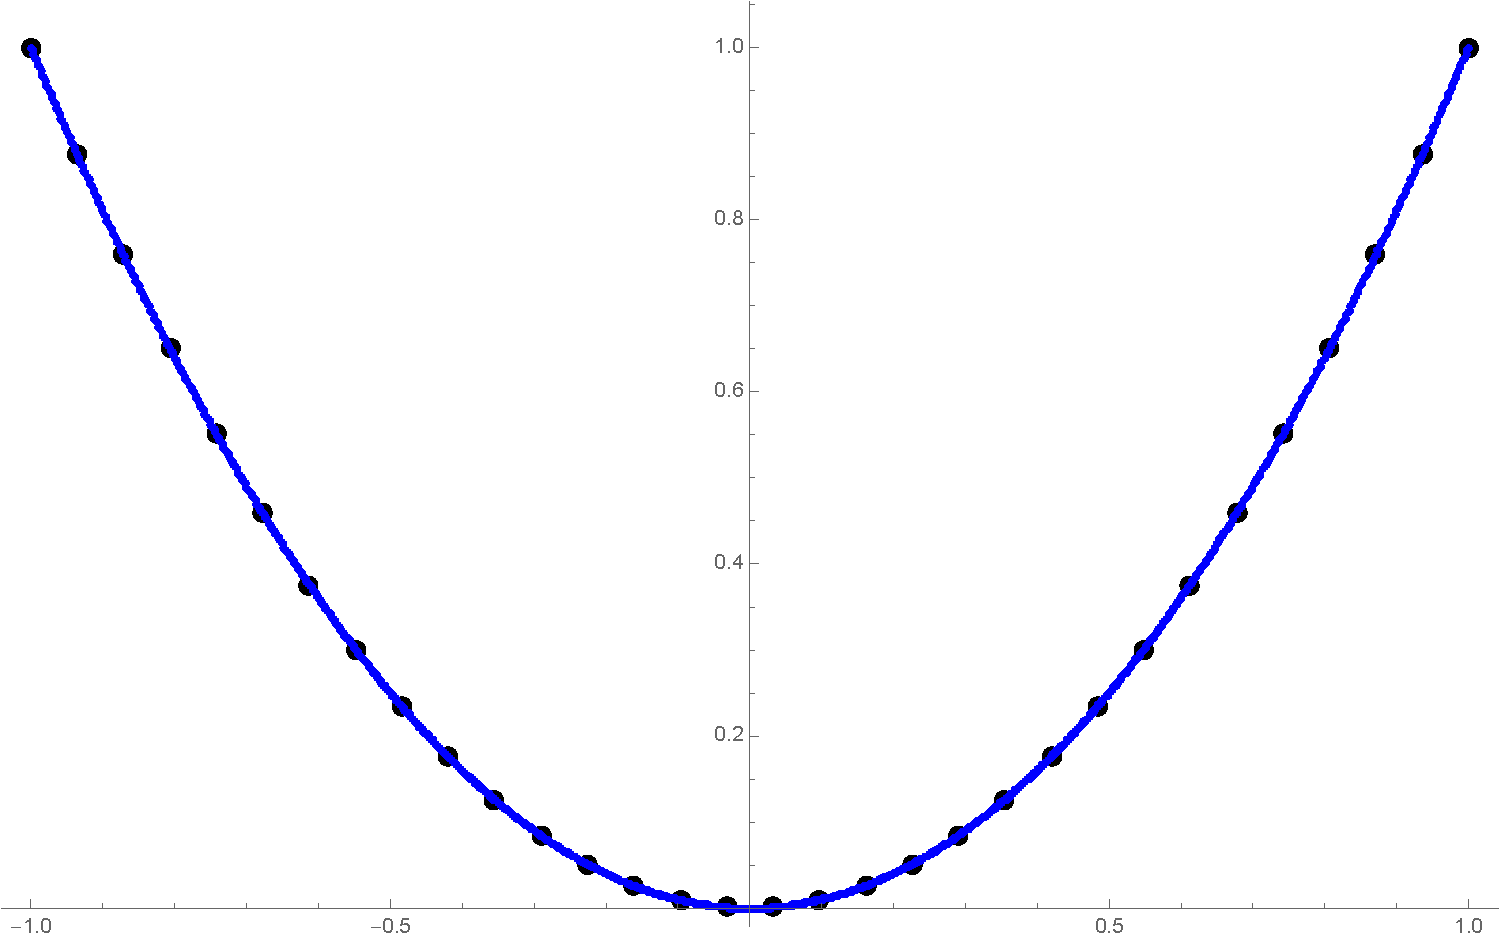
\includegraphics[width=0.8\linewidth]{pic/4/g_n_32_U.pdf}}
    \caption{Равномерная сетка, $g(x) = x^2$, $n = 32$.}
\end{figure}

\pagebreak


\begin{figure}[h]
    \center{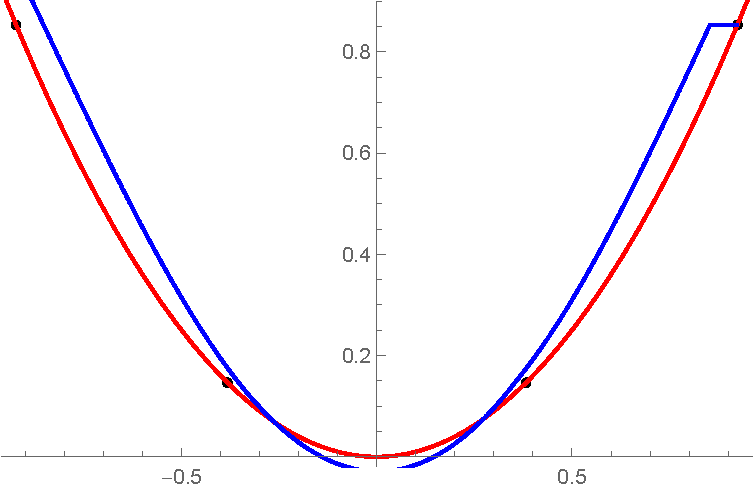
\includegraphics[width=0.8\linewidth]{pic/4/g_n_4_C.pdf}}
    \caption{Чебышевская сетка, $g(x) = x^2$, $n = 4$.}
\end{figure}

\begin{figure}[h]
    \center{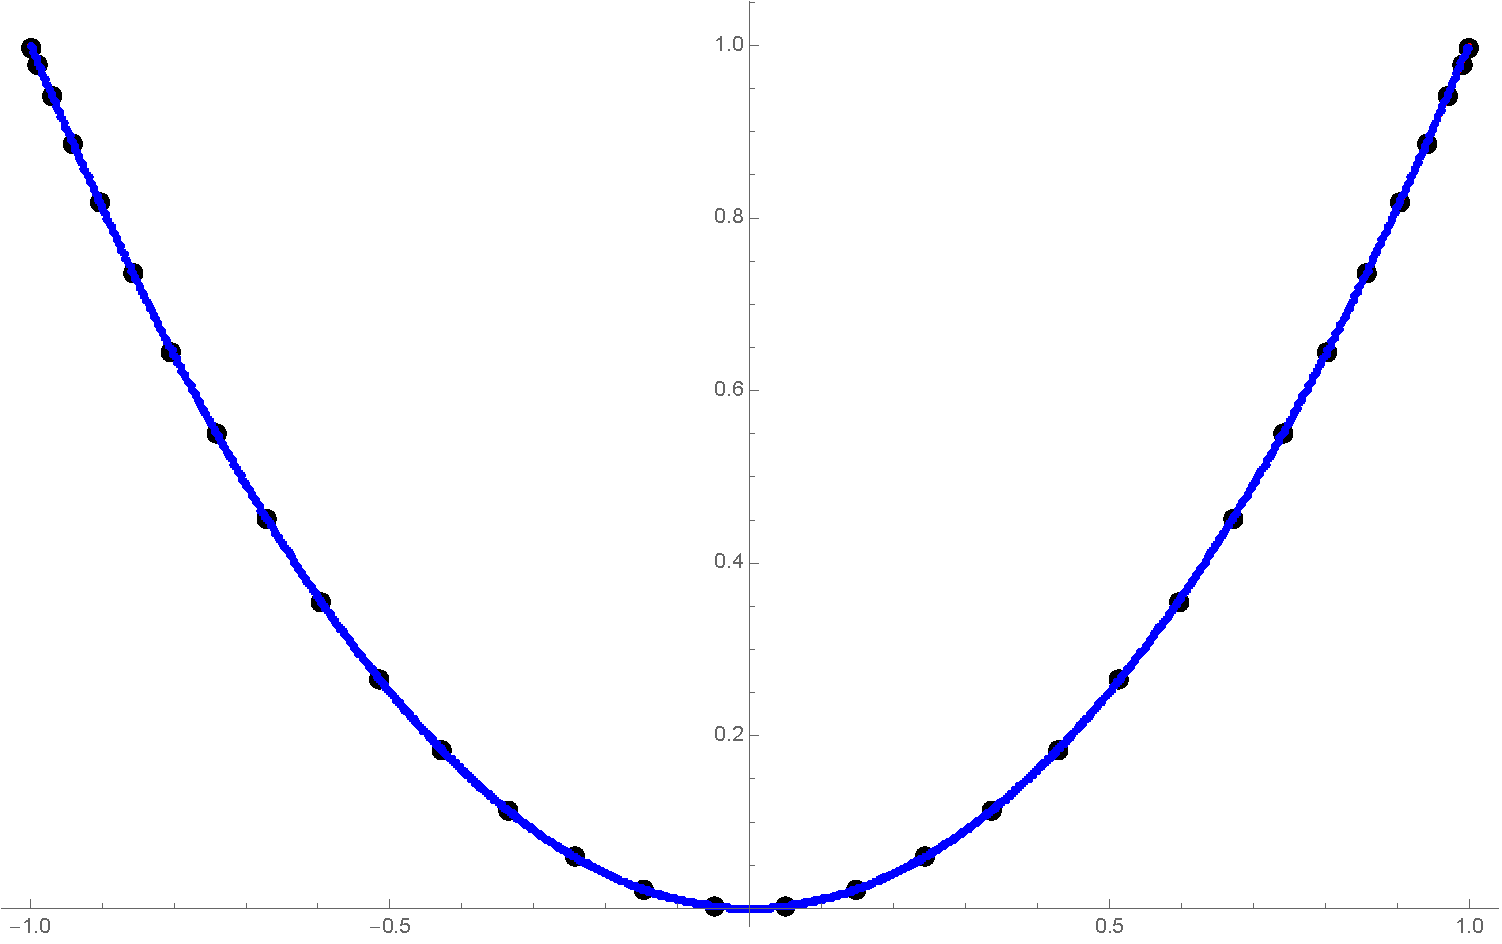
\includegraphics[width=0.8\linewidth]{pic/4/g_n_32_C.pdf}}
    \caption{Чебышевская сетка, $g(x) = x^2$, $n = 32$.}
\end{figure}

\pagebreak

\section{Контрольные вопросы}
\begin{enumerate}

\item Определите количество арифметических операций, требуемое для интерполирования функции в некоторой точке многочленом Лагранжа (включая построение самого многочлена) на сетке с числом узлов, равным $n$.

Пусть количество узлов равно $n$. Интерполяционный полином Лагранжа выглядит следующим образом:\\
$$L(x)=\sum \limits_{k=0}^{n-1} c_k(x) y_k,$$\\ где $y_k$ --- значение функции в точке $x_k$, а $c_k = \prod \limits_{j=0,k\neq j }^{n-1}\frac{x-x_j}{x_k-x_j}.$\\
Вычисление арифметических операций.

Начнем с коэффициентов $c_k$: нужна 1 операция деления, всего их будет $n-1$, и $n-2$ операции перемножения дробей. Таким образом, на вычисление каждого $c_k$ требуется $2n-3$ операций. После вычисления коэффициентов $c_k$, нужно умножить на $y_k$, т.е. еще 1 операция умножения. И все это суммируется от $0$ до $n-1$, т.е. $n-1-0+1=n$.\\
В итоге получаем: $((2n-3)+1)n = (2 n -2)n=2n^2-2n$ $\Rightarrow$ Всего для интерполирования функции в некоторой точке многочленом Лагранжа требуется $2n^2-2n$ мультипликативных операций.


Для того, чтобы посчитать коэффициент $c_k(x)$ и умножить его на $y_k$, нужно $n$ операций. Для подсчета суммы всех произведений $k = \overline{1,..., n}$ нужно $n \cdot n = n^2$ операций.

\item Определите количество арифметических операций, требуемое для интерполирования функции в некоторой точке кубическим сплайном (включая затраты на вычисление коэффициентов сплайна) на сетке с числом узлов, равным $n$.

Для подсчета $g_i$ нужно $n$ операций. Для прогонки потребуется $5n$ операций. Далее для подсчета коэффициентов $b_i$ и $d_i$ нужно $3n + 2n = 5n$ операций. Итог: $n + 5n + 5n = 11n$.

\pagebreak

\item Функция $f(x) = e^x$ интерполируется многочленом Лагранжа на отрезке $[0, 2]$ на равномерной сетке с шагом $h = 0{.}2$. Оцените ошибку экстраполяции в точке $x = 2{.}2$, построив многочлен Лагранжа и подставив в него это значение, а также по формуле для погрешности экстраполяции.

\begin{figure}[H]
    \center{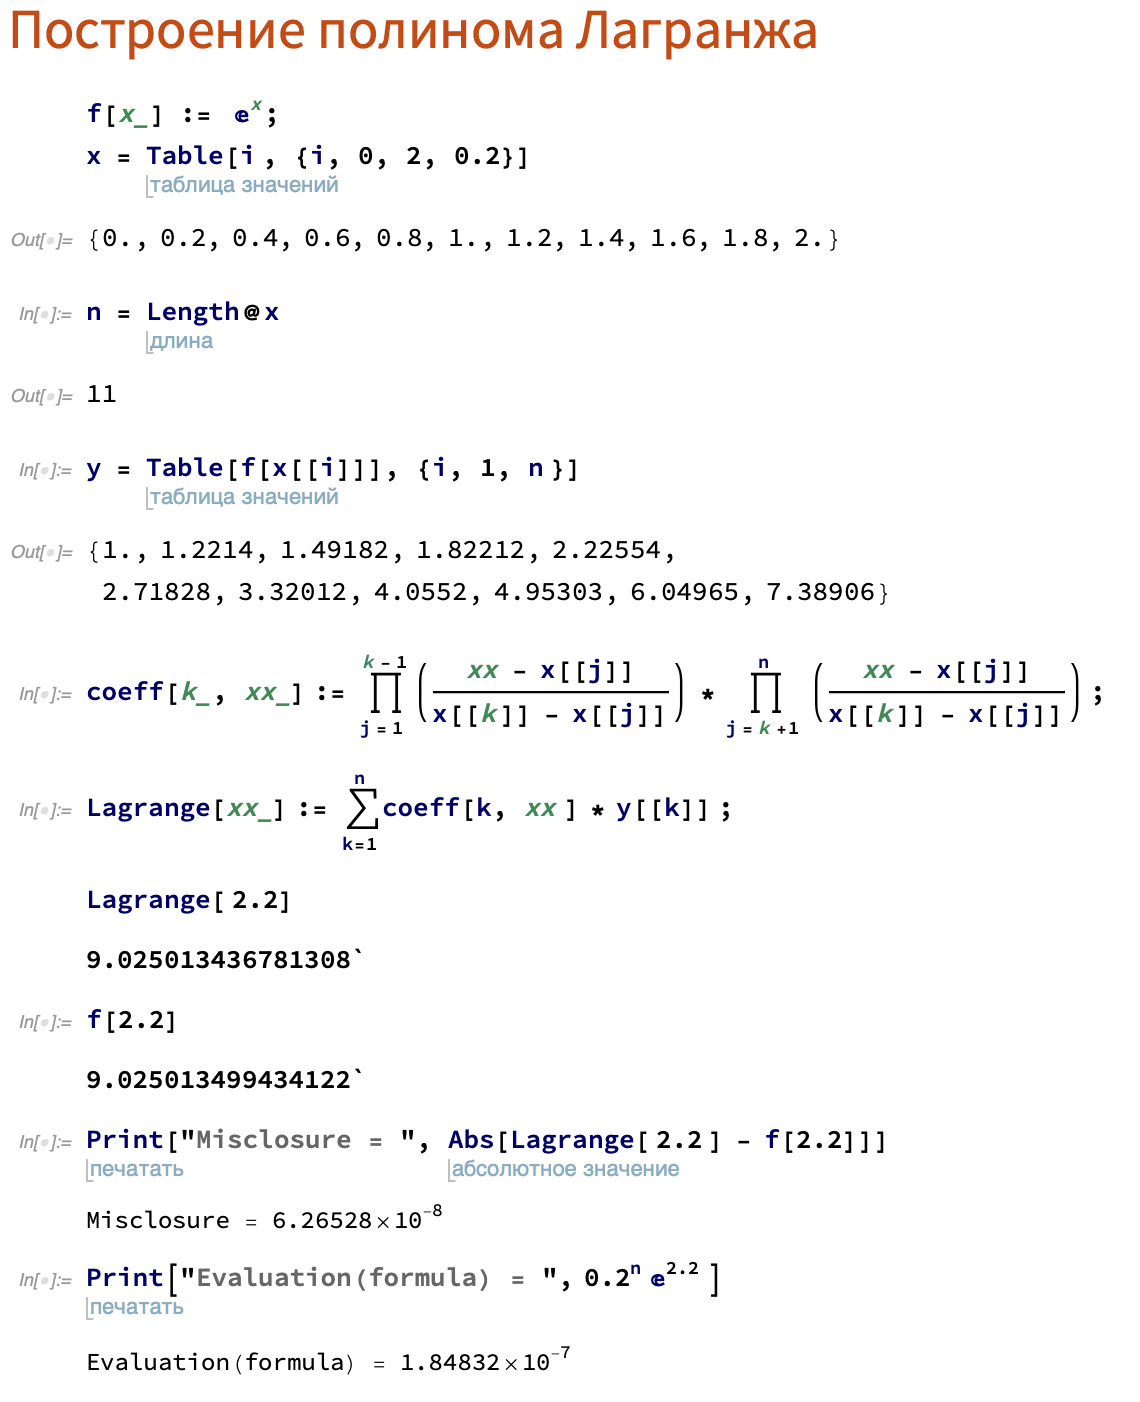
\includegraphics[scale=0.7]{pic/misclosure.png}}
    \caption{Полином Лагранжа для функции $Exp[x]$. Нахождение значения этого полинома в точке $ x = 2.2 $. Сравнение с оценочной формулой}
    \label{fig:misclosure}
\end{figure}

\pagebreak

\item Выпишите уравнения для параметров кубического сплайна, если в узлах $x_0$ и $x_n$ помимо значений функции $y_0$ и $y_n$ заданы первые производные $y'(x_0)$ и $y'(x_n)$.

\item Каковы достоинства и недостатки сплайн-интерполяции и интерполяции многочленом Лагранжа?

{\bf Интерполирование многочленом лагранжа.} \\ $+\colon$ график интерполяционного многочлена Лагранжа проходит через каждую точку массива, конструируемая функция легко описывается (число подлежащих определению коэффициентов интерполяционного многочлена Лагранжа на сетке равно $n+1$), построенная функция имеет непрерывные производные любого порядка, заданным массивом интерполяционный многочлен определен однозначно. \\ $-\colon$ погрешности вычислений, неустойчивость для большого количества узлов, степень многочлена зависит от узлов сетки, необходимость все пересчитывать при добавлении нового узла.
\\
{\bf Интерполирование сплайнами.} \\ $+\colon$ график построенной функции проходит через каждую точку массива, конструируемая функция сравнительно легко описывается, степени многочленов не зависят от числа узлов сетки и, следовательно, не изменяются при его увеличении, построенная функция имеет непрерывные производные. \\ $-\colon$ осцилляция в окрестности точки, сильно отличающейся от соседних

\item Какие свойства полиномов Чебышева и чебышевских сеток Вам известны?
\begin{enumerate}
    \item Многочлен Чебышева первого рода $T_n(x)$ характеризуется, как многочлен степени $n$ со старшим коэффициентом $2^{n + 1}$, который меньше всего отклоняется от нуля на отрезке $[-1, 1]$
    \item Многочлен Чебышева второго рода $U_n(x)$ характеризуется, как многочлен степени $n$ со старшим коэффициентом $2^{n}$, интеграл от абсолютной величины которого по отрезку $[-1, 1]$ принимает наименьшее значение. 
    \item Многочлены четных степеней являются четными функциями, нечетных степеней являются нечетными функциями, то есть при четном $n$ многочлен $T_n(x)$ содержит только четные степени $x$ и яляется четной функцией, а при нечетном $n$ многочлен $T_n(x)$ содержит только нечетные степени $x$ и является нечетной функцией.
\end{enumerate}


\end{enumerate}
\newpage

\end{document} 